% This file is part of the Apogee project.
% Copyright 2014 Melissa Ness and David W. Hogg.

% # short-term to-do
% - finish first draft
% - send out to \apogee\ collab for comments.

% # style notes
% - are they ``labels'' or ``labels''?  MKN:  Make a call and audit the whole text.
% - needs a name and to use it consistently as \thename

\documentclass[12pt, preprint]{aastex}
\usepackage{bm, graphicx, subfigure, amsmath, morefloats}
\input{vc}
\newcommand{\sectionname}{Section}
\newcommand{\documentname}{\textsl{Note}}

%\usepackage{natbib}
\bibliographystyle{apj}

\newcommand{\set}[1]{\bm{#1}}
\newcommand{\mean}[1]{\overline{#1}}
\newcommand{\given}{\,|\,}
\newcommand{\teff}{\mbox{$\rm T_{eff}$}}
\newcommand{\kms}{\mbox{$\rm kms^{-1}$}}
\newcommand{\feh}{\mbox{$\rm [Fe/H]$}}
\newcommand{\logg}{\mbox{$\rm \log g$}}
\newcommand{\tc}{\textsl{The~Cannon}} 
\newcommand{\apogee}{\textsl{APOGEE}} 
\newcommand{\apokasc}{\textsl{APOKASC}} 
\newcommand{\galah}{\textsl{GALAH}} 
\newcommand{\aspcap}{\textsl{ASPCAP}} 
\newcommand{\gaiaeso}{\textsl{Gaia-ESO}} 
\newcommand{\gaia}{\textsl{GAIA}} 
\newcommand{\matisse}{\textsl{MATISSE}} 
\newcommand{\rotwarn}{\texttt{ROTATION WARNING}} 
\newcommand{\sdss}{\textsl{SDSS-III}} 
\newcommand{\aspcapstar}{\textsl{aspcapStar}} 
\newcommand{\apstar}{\textsl{apStar}} 


\begin{document}

\title{\textsc{\tc:}\\ A data-driven model for stellar parameter determination}
\author{
  MKN,
  DWH,
  \&
  HWR,
  AH, GZ} 
\date{DRAFT / NOT FOR DISTRIBUTION}



\begin{abstract}%
New spectroscopic surveys offer the promise of consistent stellar
parameters and abundances (`stellar labels') for hundreds of thousands
of stars in the Milky Way. 
These labels are currently derived by comparisons with physics-based
model spectra, which are technically challenging, and often use only a
modest fraction of the spectral pixels. 
In many cases, however, there is a sub-set of \emph{reference}
objects for which the stellar labels are known with high(er)
fidelity; this is the use case for \tc.
From the reference stars, \tc\ learns (by fitting a very flexible
model) how the flux in each pixel of a continuum-normalized spectrum
depends on the `known' stellar labels; \tc\ then exploits this same
dependence to derive new labels for the non-refererence stars.
We illustrate \tc\ by applying it to the spectra of 59,000 stars from
\apogee\ DR10. 
We take \teff, \logg\ and \feh\ as the labels, and 545 stars in 19
clusters as the reference objects (training set). 
\tc\ is very accurate; its stellar labels compare well to the 37,500
stars for which \apogee\ pipeline (\aspcap) labels are provided; we
obtain rms differences of $\delta\teff< 100$~K, $\delta\logg< 0.2$~dex
and $\delta\feh< 0.1$~dex.
Aside from the modeling of the training-set stars (which could happen
in another dataset or at another wavelength), \tc\ makes no use of
stellar models nor any linelist; its biggest limitation is that it
requires a training set that spans the label-space. 
The method degrades very weakly with signal-to-noise; \tc\ delivers
the labels with good fidelity even at one ninth the
\apogee\ observing time. 
We discuss the limitations of \tc, and point out the potential of this
approach to bring different spectroscopic surveys onto a consistent
scale of stellar labels if they have sufficient objects in common.
\end{abstract}

\keywords{%
methods: data analysis
---
methods: statistical
---
stars: abundances
---
stars: fundamental parameters
---
surveys
---
techniques: spectroscopic
}

\section{Introduction}

The vast spectroscopic stellar surveys of recent years (REFs to: SEGUE, RAVE, LAMOST, APOGEE, Gaia-ESO, Galah) hold tremendous astrophysical promise, but at the same time present formidable data analysis and modeling challenges. 
One of these challenges lies in consistently and accurately determining stellar labels, that is, stellar parameters and element abundances, from survey spectra. 
These labels are usually determined from comparison of the data with synthetic model spectra, with approaches often 
customised specifically to the particular wavelength region of a given survey (REF to APOGEE, SEGUE, RAVE \& Gaia-ESO pipeline papers). 
The stellar photosphere models that are relied upon for stellar label determination have physical ingredients that are incomplete and simplified. 
For computational feasibility, almost always 1D stellar photosphere models are adopted for large surveys, often assumed to be in local thermal equilibrium. 
In many cases, the model spectra do not account for all relevant  molecular opacities, for convection, stellar winds and for the stellar chromosphere. 
As a consequence, it happens that different research groups obtain discrepant results even for the same data on the same stars, due to different input assumptions and methods \citep[e.g.]{Sm2014}. 

Stellar labels are commonly determined by fitting a model spectrum (with known labels) to the data using some minimisation technique, often restricted to a masked portion of the spectrum that is focussed on the absorption line (regions) deemed to be most reliable or relevant. 
Stated minimal signal-to-noise requirement to obtain robust labels in this way are $S/N\sim 100$ per resolution element, especially if the labels are to include individual element abundances. 
Often, a post-calibration procedure is applied to bring the stellar labels derived by such a fitting pipeline in accord with external information of higher fidelity: for example with stellar labels from benchmark stars studied at high resolution and/or well characterised open and globular cluster stars (REF: which surveys have done that?). 

In practice, different surveys end up having different calibrations of their labels: either their stellar parameter or their abundances are on slightly different scales; this complicates
inter-survey comparisons and constitutes major challenge of the era of such large datasets. 

In this paper we propose and lay out a data-driven approach to deriving stellar labels from stellar spectra in the context of large spectroscopic surveys, which we dub \tc\footnote{why it is called the Cannon}. 
The main practical strengths of \tc\ lie in the fact that it is enormously fast, it can obtain labels of comparable accuracy to quoted in current approaches but with far less S/N, and it offers a consistent way to cross-calibrate surveys. 
To do so, \tc\ must rely on the existence of a subset of objects within a survey
(\textit{reference objects}), for which the stellar labels are known sufficiently well and cover label space sufficiently.

In this context, the term {\sl labels} refers to the pieces of information that characterize and determine a stellar spectrum; these labels are commonly and sensibly split into {\sl stellar parameters} and {\sl element abundances}, though in the context of \tc\ it makes sense to treat them on a par. 
In most cases, it suffices to think of the labels as \teff , \logg, and the element abundances [X/H], though stellar rotation, microturbulence, etc.. can also be thought of as labels. It is central to the approach we lay out here that stars with the same labels have (nearly) identical spectra and that spectra vary smoothly with label changes. 
This must be true, if the set of labels is comprehensive enough so that it fully specifies the star; but if the labels are e.g. only \teff, \logg \feh\ then this is obviously an approximation. 

There are fundamentally two steps in \tc . 
The first step in \tc\ is to create from the spectra of the \textit{reference objects} a generative model that describes the flux at every pixel in their continuum normalized spectra as a function of their known stellar labels. 
The second step assumes that this same generative model  holds for all the other objects in the survey (dubbed \textit{survey objects}). 
Then, the spectra of the \textit{survey objects} and the generative model from the \textit{reference objects}
allow us to solve for the labels of the \textit{survey objects}. This second step we call ``\textit{label transfer}''.

To make such an approach straigtforward, we must assume that the \textit{reference objects} and the \textit{survey objects} were observed with the identical instrumental set-up, a condition well satisfied with the large surveys listed above. 
We take the generative model for the continuum normalized flux at each of $N_{pix}$ pixels to be a polynomial function of all the labels, and hence the model is defined by its $N_{pix}$ sets of polynomial coefficients. In practice, there may be different circumstances that make stars suitable reference objects. 
They may be members of star clusters: there, external data and the fact that clusters are in good approximation single stellar populations (which have to fall onto an isochrone) lend credibility to their stellar labels. 
Alternatively, reference objects could be stars for which labels have been derived separately from spectra of particularly high signal to noise, or at other "easier" or more extensive wavelength regimes (e.g. in the optical as opposed to the IR). 
Finally, they may be subsets of stars in a survey  for whom other approaches to get stellar parameters (e.g. astroseismology ) may provide accurate stellar parameters.

With this two-step procedure of training on spectra of reference objects and then transferring the label information to the survey objects, \tc\ falls into the class of \emph{supervised methods} in machine learning. 
However, what we implement is very different in a crucial way from standard supervised methods for regression, such as support vector machines, random forests, and deep learning.
These other methods also try to fit a very flexible model to the training data at training time
and deploy that model on the test data at test time.
The important difference, however, is that \tc\ is a \emph{generative model} of the observed spectra:
That is, it constructs, as a function of labels, a probability density function (pdf) for the observed
flux as a function of wavelength. 
This makes \tc\ a bespoke method, not cleanly falling into any established machine-learning methodology.
However, it gives us the enormous advantage that we can account for the uncertainties in the spectral data,
including all the issues of heteroscedasticity and missing data.
It also makes the method agnostic about signal-to-noise.
This point is technical, but important:
In many real cases the training data will be much higher in signal-to-noise than the test data
(standard stars tend to be bright and well observed).
A method that does not properly account for the observational uncertainties will not transfer labels to lower signal-to-noise spectra with high fidelity.
In what follows, we show that \tc\ behaves very well as the signal-to-noise (or observing time) is decreased.

In this paper we use \apogee\ as the sole example. 
However, \tc\ can be applied to any stellar survey.  
Our aim is distinct from simply determining parameters or finding the best fit spectra similarly to minimisation techniques. 
Our aim is to implement a procedure which makes it possible to understand and characterise the spectra as a function of the labels which describe it.  
Our methodology is very relevant for chemical tagging in large datasets, as it can formally describe and differentiate the spectra in multiple-abundance space, given additional input labels.
In the same way it is possible to implement a differential analysis on large datasets using this approach. 
Our most basic implementation of \tc\ that we present includes only three labels, but this can easily be extended to additional labels  (e.g. [$\alpha$/Fe], [X/Fe]) and also more comprehensive models (e.g. Gaussian processes). 
Additionally, as we are using the information in every pixel, this methodology is effective at determining labels at lower signal to noise (SNR) than minimisation techniques.% and provide a quantification of data-driven spectra comparison and differentiation, which may be a key tool in exploring the archeology of stars via chemical tagging. 

Our overarching aim of describing stellar flux as a function of stellar labels is not dissimilar from the MATrix Inversion for Spectral SythEsis (\matisse) procedure for derivation of stellar parameters \citep{RB2006}. 
However, \matisse\ employs a large grid of synthetic spectra and characterises a set of basis vectors which project onto each observed spectrum to determine stellar labels by calculating an optimal combined synthetic spectrum describing the stellar flux. 
Conversely, we use a data-driven model and do not project onto any optimal combined theoretical spectrum. 
Rather we directly determine labels using a total of around 70,000 degrees of freedom of information in the data, given the 7200 pixels comprising the flux and the 10 parameters of the labels in our implemented model. 

We have adopted a bottom-up approach for \tc\ , starting with the most basic implementation and successively adding complexity to the generative model to determine the least complex implementation which works.  
In laying out the methodology of this approach we firstly describe the \apogee\ dataset and the way we process the data for both reference objects (545 stars) and survey objects ($\sim$ 59,000 stars from DR10). 
We then describe perhaps the simplest implementation of label-transfer possible, using a first-order linear model. We found this first-order model to be insufficiently flexible to describe the labels of the stars and so we extended our model to quadratic form, which satisfactorily describes the label-space of the training data.
The success of this model is demonstrated by running \tc\ through the DR10 data available through the SDSS-3 data server, the results for which we provide in an online machine-readable table. % for about 42,000 DR10 stars. 

\section{Data}

Our approach \tc \ is applicable to any large, homogeneous spectroscopic data set. Here, we use the \apogee\ data to showcase \tc . 
We describe how we prepare the data for the reference objects, to prepare the label-transfer and similarly, how to process the survey data.

\subsection{Reference objects with high-fidelity stellar labels}

The first step in \tc\ is to chose a set of reference (or training) objects for which we have spectra from the survey and 
\emph{also} high-fidelity labels (i.e. stellar parameters and element abundances that are deemed both accurate and precise). 
The set of reference objects is critical, as the subsequent label transfer to the survey objects can only be as good as the quality 
of the reference labels. 
Also, as \tc\ may have to inter- and extrapolate to new parts of label space as
it encounters new kinds of spectra among the survey objects, the quality
of the label transfer depends on the density and extent to which the reference objects
cover label space (\teff, \logg, [Fe/H], [X/Fe], and so on). 
The performance of data-driven model like \tc\ can depend strongly on the size and quality of its set of reference objects.

Any set of reference objects in the survey with high fidelity labels is good for the implementation of \tc.
In practice, a set of reference objects that satisfies these criteria (e.g. in \apogee )
consist of members of well studied open and globular clusters that have their labels derived from high resolution spectral analysis in the
optical wavelength region.

Specifically, the reference dataset we use is that of the globular and open cluster data observed by \apogee\ for calibration of their abundance pipeline \citep{Meszaros2013}. 
This reference dataset is comprised of about 545 stars from 19 open and globular clusters, which span stellar parameter ranges 
of 3500 $<$ \teff\ $<$ 5300, 0 $<$ \logg\ $<$ 5 and --2.5 $<$ [Fe/H] $<$ 0.45. 
Exactly which stellar labels we adopt for theses reference objects, is critical to the subsequent output, and hence we discuss it in detail here.

% note there are 20 in their list but 1 gc has only 1 star and the abundance looks incorrect to me. 

We adopt the DR10 ``\aspcap\ corrected'' stellar parameters for each of those 545 stars as their labels, 
which will then place the output from \tc\ for the survey objects after label transfer on the \apogee\ \aspcap\ scale.
 This set of stars is the very same stars used by \apogee\ to post-calibrate the output of \aspcap\ to a physical stellar parameter scale \citep{Meszaros2013}.
Adopting the \aspcap\ corrected labels provided and documented by \apogee\ has the important advantage 
that we can test exactly how well we can reproduce the results from \apogee\ for the survey stars via label-transfer of only 545 stars.

The corrections to the labels made by \apogee\ based on the cluster data are applied to the immediate output of the \aspcap\ pipeline that arose from comparisons to a library of stellar models.
Temperature corrections are determined by comparing the infrared flux temperatures of the stars \citep{gonzalez2009}, \logg\ corrections are from the offset between \aspcap\ results and Kepler results for common stars and \feh\ corrections are from the difference between the \aspcap\ and  the literature value of each cluster.  
The \apogee\ corrections determined in \citet{Meszaros2013} are valid only for stars with \logg\ $<$ 3.5 and are not implemented for the dwarfs.  We adopt the \aspcap\ corrected [M/H] values for these clusters and these are corrected to the [Fe/H] of the clusters and so we adopt this label as an [Fe/H] (that is, this label from \apogee\ therefore, does not explicitly use \feh\ lines, but is derived from an \feh\ correction). 
The analysis in \citet{Meszaros2013} is restricted not only to giants but also stars with SNR $>$ 70, determined to be the minimum SNR for reliable stellar parameters by \apogee.

These corrections implemented by \apogee\ in \teff, \logg\ and  \feh\ place the giants in the cluster stars on or near the iscohrones (see Figures 7 and 8 in Meszaros et al., (2013)).  
As there are no \aspcap\ corrections implemented for the few main sequence stars among the reference objects, 
we instead determine temperatures for these dwarfs, which are all in the Pleiades, directly using same correction method 
as in \citet{Meszaros2013}. 
We determine the infrared flux temperature for the stars from \citet{gonzalez2009} and apply a correction to 
the \aspcap\ output based on the offset in the temperature scales. We find the following relation:
 $T_{\mbox{corrected}}$= 0.855*T$_{\mbox{\textit{\aspcap}}}$ + 1206.7.


We do not attempt an individual metallicity correction for each dwarf star but rather set all \feh\ of the dwarf spectra to \feh\ = 0.03 \citep{barrado2001}.
Tests on the input labels to \tc\ demonstrate that there is only a small degradation of the results caused by adopting a single \feh\ for every cluster star for the literature value of the cluster, instead of individual \feh\ values for the stars (that is, from the \aspcap\ corrected values). 
To determine the \logg\ for these Pleiades main sequence stars, we shift the stars vertically to their nearest positions on an appropriate age-metallicity Padova isochrone of 150 Myr at [Fe/H] = 0.03 \citep{girardi2000}. 
Due to the high differential reddening to the Pleiades, and the subsequent large temperature errors using the IR flux method that result from this, we only selected the 64 from a total of 72 Pleiades dwarfs, eliminating those with high extinction of SFD (corrected) E(J-K) $>$ 0.30 \citep{Schlafly2011}.

Adopting the input labels from the \aspcap-corrected parameters determined from calibrations to literature cluster values also transfers the errors from the \aspcap\ pipeline: of $<$ 150K in \teff,  $<$ 0.2 dex in \logg\ and $<$ 0.1 dex in \feh.   
The uncertainties on the input labels will be included as an input parameter of the labels in a future development stage of \tc. Inclusion of uncertainties may be particularly relevant when introducing multiple labels of individual elements. 

For a comparative analysis to the ``\aspcap\ corrected'' labels, we adopt a \logg\ label for all of the training stars not from the Kepler scale, but rather from the best vertical fits to the isochrone for the ages and metallicities for the clusters from the literature (with the temperatures fixed). 
We call these the ``Isochrone-corrected labels'', where we use Padova isochrones at the age and \feh\ of each cluster. 

The above set of labels for the reference objects is well defined, but still means that the reference objects in the clusters do not lie on a single model isochrone 
(see Fig. \ref{fig:trainingaspcap}). 
As an alternative set of reference labels, we consider one where the stellar parameters (\teff , \logg ) of the reference objects lie by construction on a single isochrone. 
For that we adopt a \logg\ label for all of the reference stars not from the Kepler scale, but rather from the best vertical fits to the isochrone for the ages and metallicities for the clusters from the literature (with the temperatures fixed). We call these the ``Isochrone-corrected labels'', where we use Padova isochrones at the literature age and \feh\ of each cluster. 

We discuss our motivation for doing this and our results in the Discussion section of our paper.  
The two calibration sets of data, the ``\aspcap-corrected'' labels and the ``Isochrone-corrected'' labels, are shown in Figures \ref{fig:trainingaspcap} and \ref{fig:trainingisochrone}, respectively. 

%run -i fitiso_apogeetempfeh_paperrework2.py
%makeonisochrone_training_4panel_revb.py
\begin{figure}[h!]
\centering
    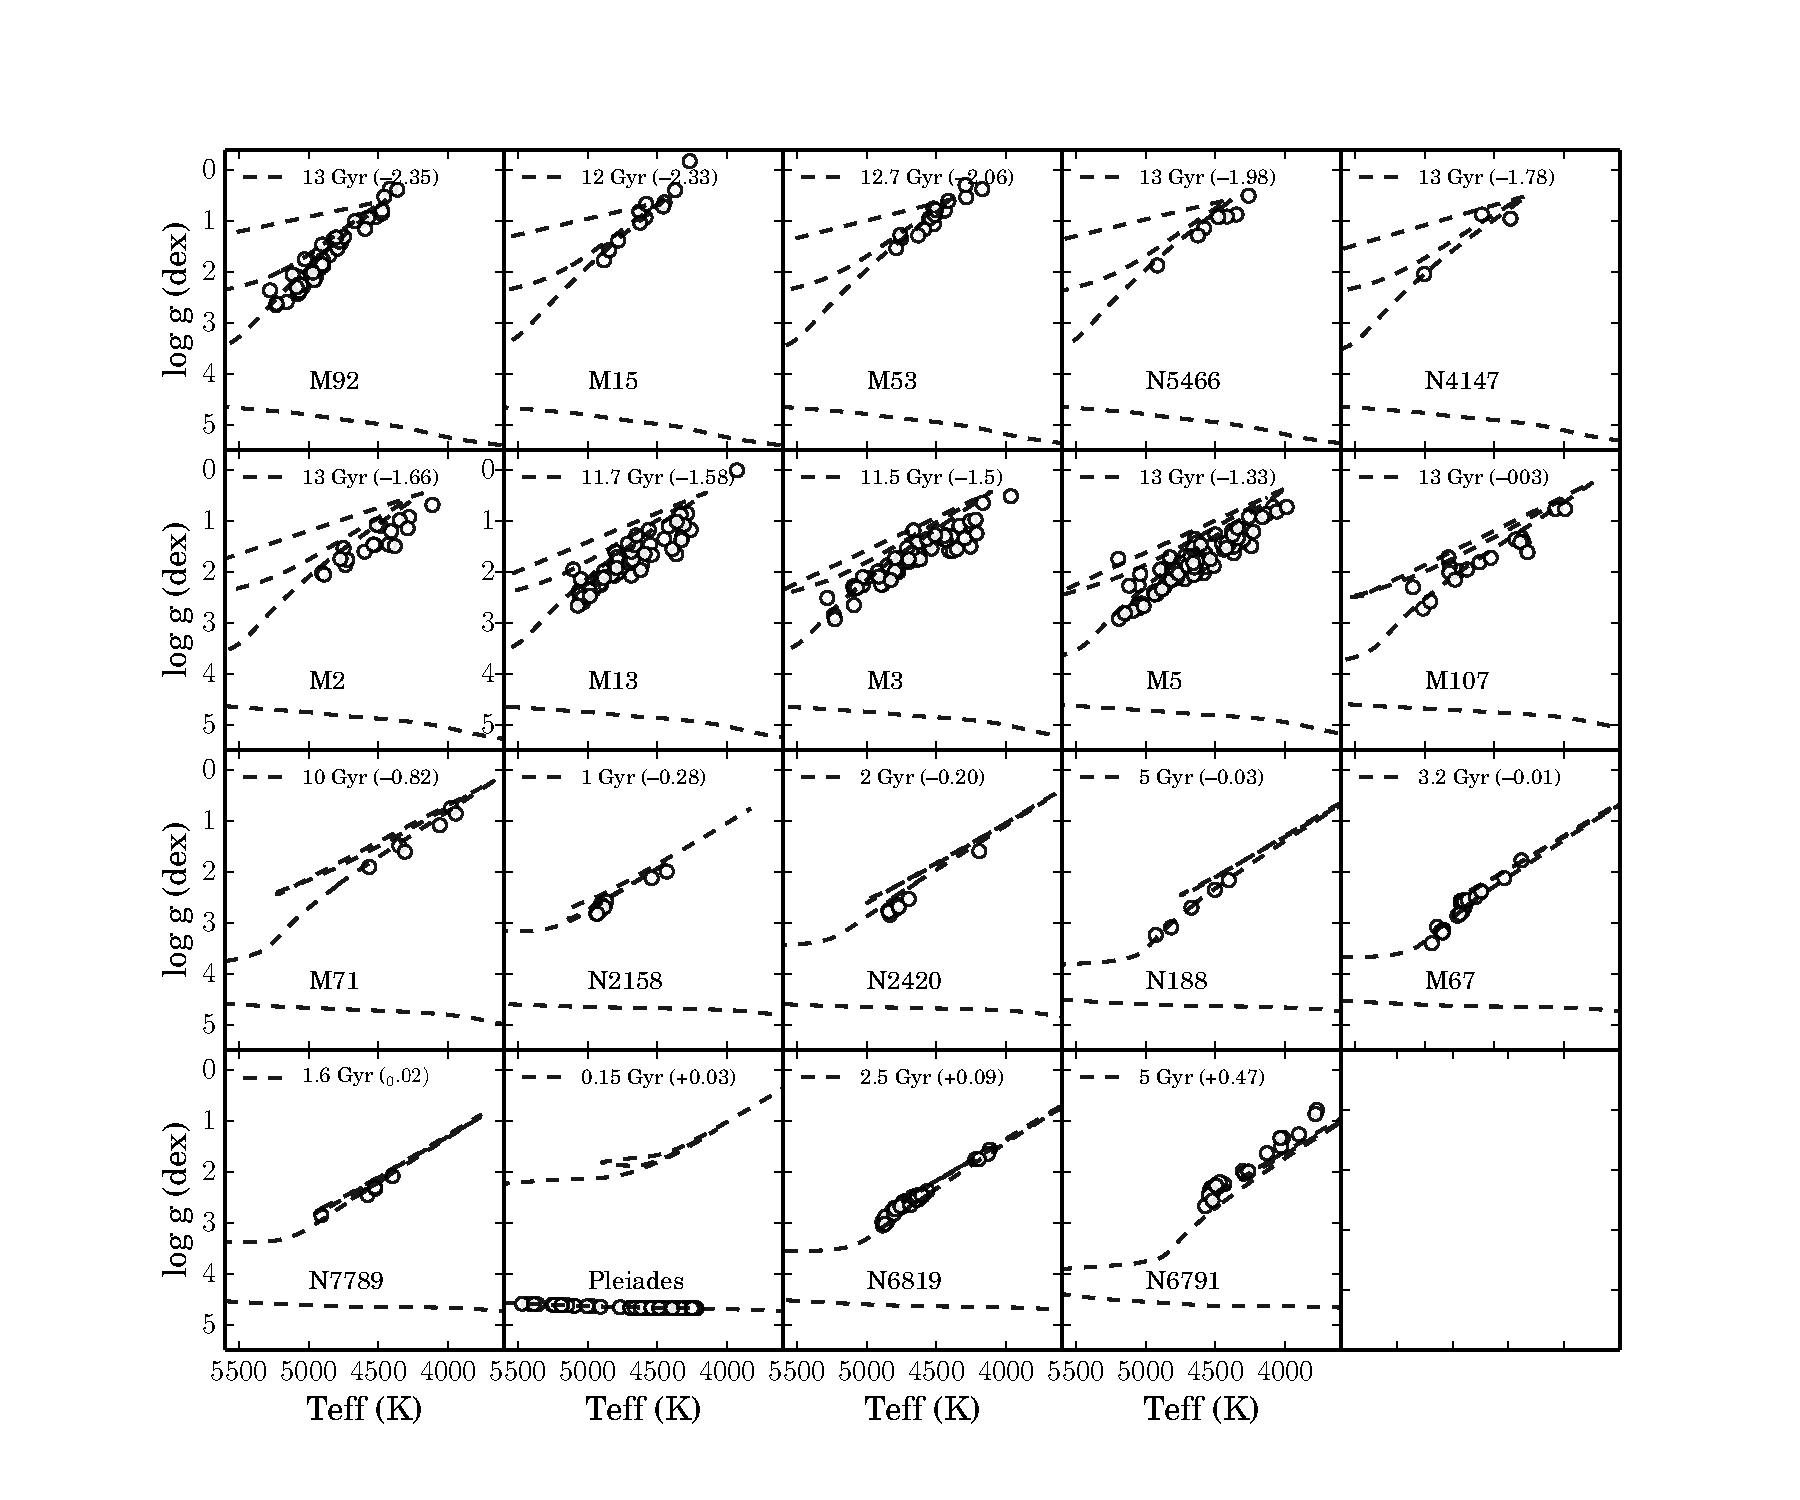
\includegraphics[scale=0.33]{./plots/training_aspcap.pdf}
\caption{\aspcap\ corrected training labels in \teff-\logg\ plane for every cluster. All labels adopted from DR10 except for the Pleiades. }
\label{fig:trainingaspcap}
\end{figure}

\begin{figure}[h!]
\centering
  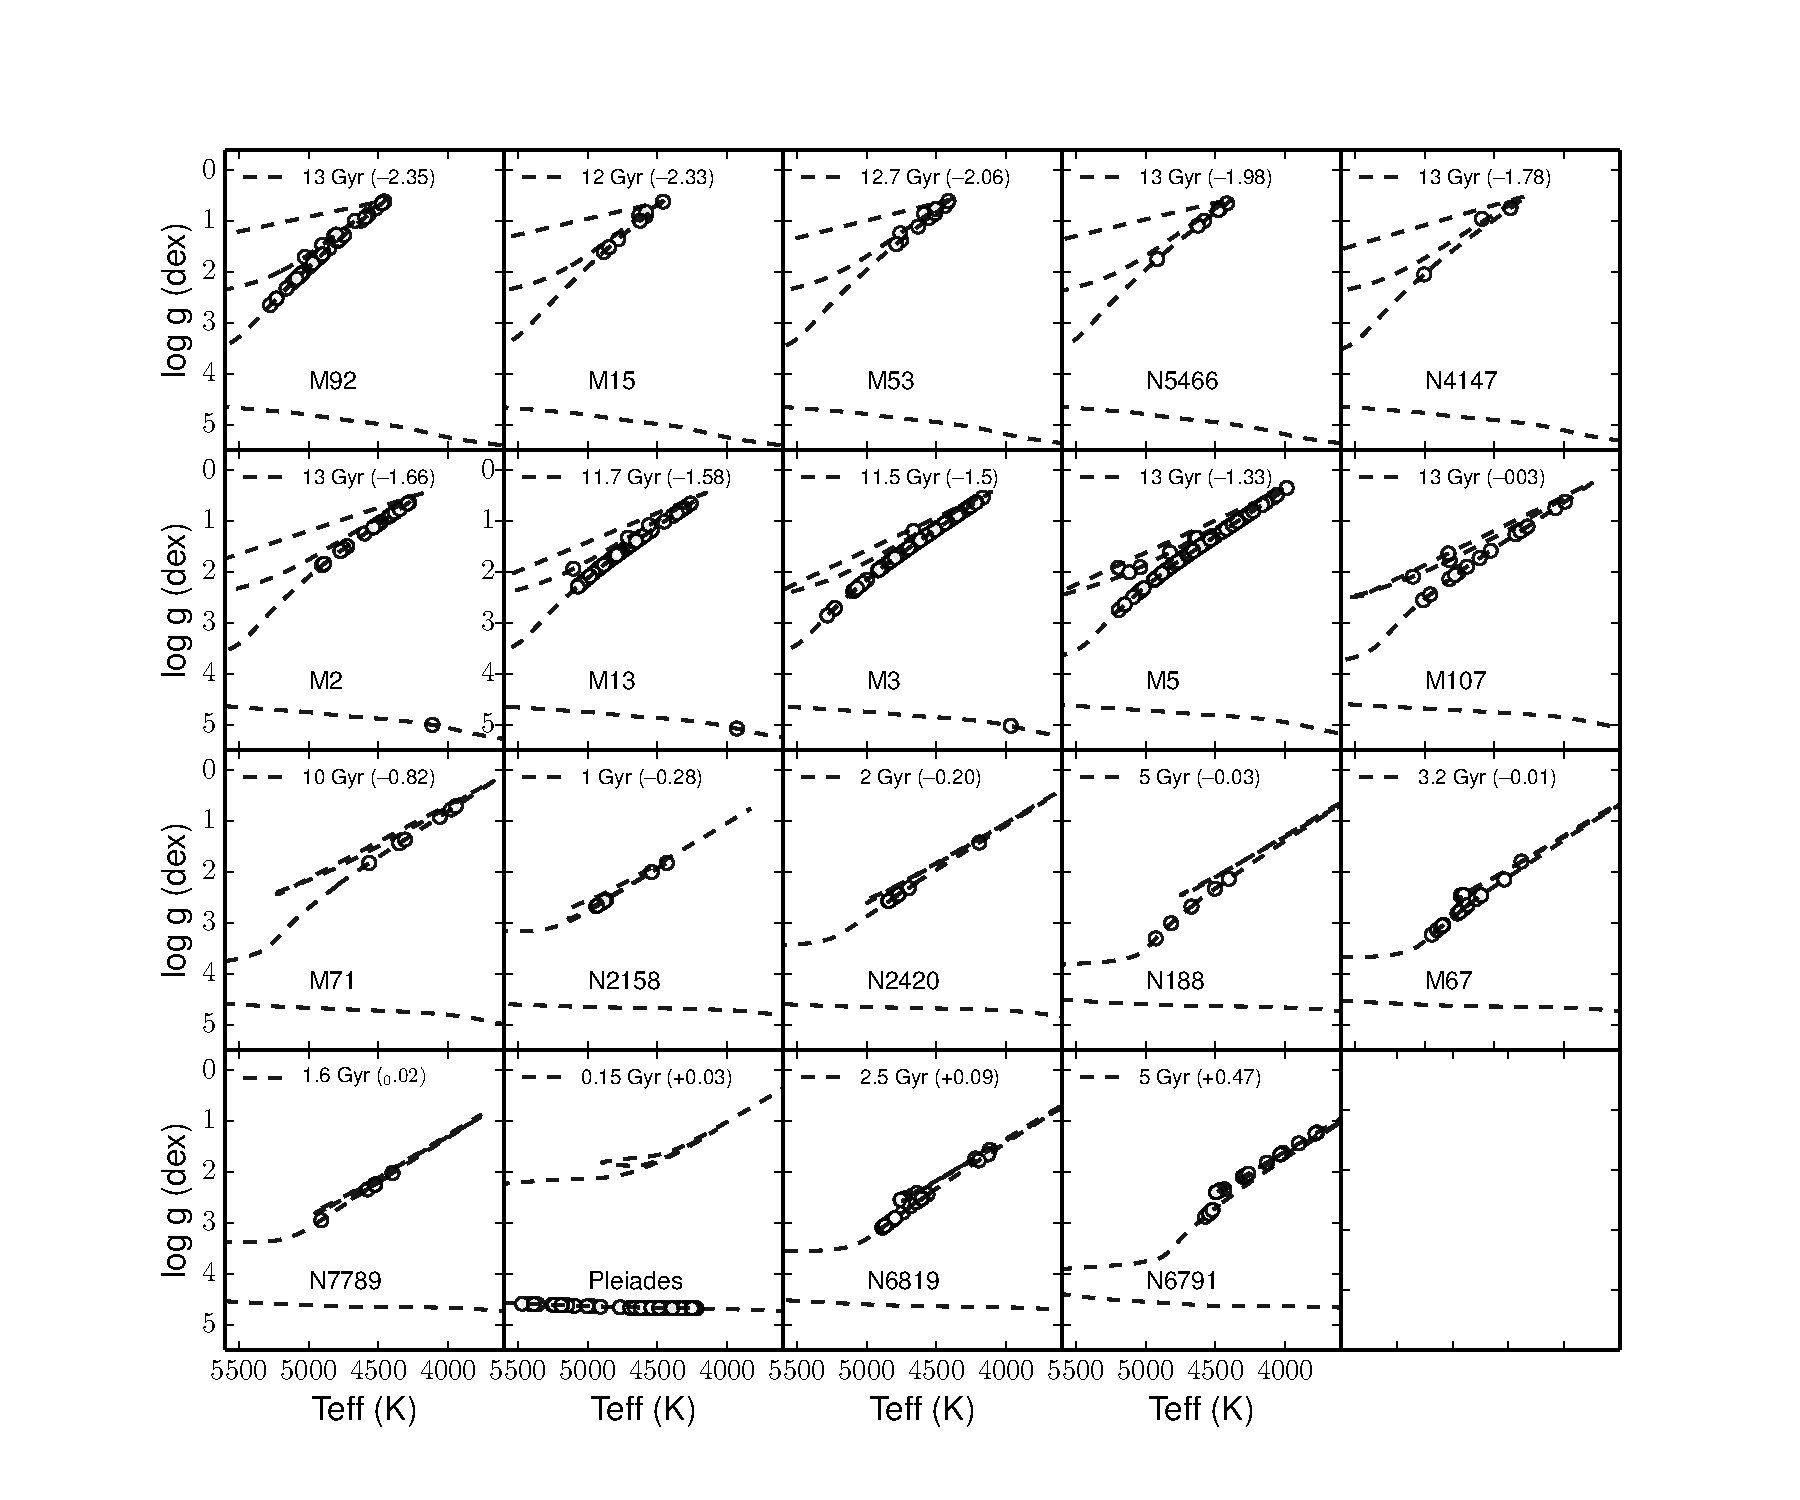
\includegraphics[scale=0.33]{./plots/training_mkn2.pdf}
\caption{Stellar labels for all reference objects as is Figure \ref{fig:trainingaspcap} except that the \logg\ values have been adjusted from the \aspcap\ value to exactly match the isochrone, we call  'isochrone-corrected' labels to differentiate this from the correction in Figure \ref{fig:trainingaspcap}.  }
\label{fig:trainingisochrone}
\end{figure}


\subsection{Continuum Normalisation and \apogee\ Test Data}

The Cannon, as we present it here, operates on continuum-normalized spectra, reduced and re-sampled to the same wavelength grid
 (with the same line-spread function), and shifted to their rest-frame. 
 Therefore, a robust continuum normalisation of the spectra is critical.
  It turns out that it is of particular importance to have an operational procedure to set the continuum,
   that shows no systematic dependence on the S/N of the spectra.

One can at first define a preliminary continuum normalisation by using polynomial fit to an upper quantile of the spectra
 in the \apogee\ pipeline \citep{Meszaros2013}. This is effective, but SNR dependent.
Then the \tc\ can provide an improved identification of continuum regions in the spectrum,
designated as those that show almost no dependence in their normalized flux on the stellar labels.
I.e. we can determine with the \tc\ the `true' continuum, using the model derived from the pseudo-continuum normalised spectra for the reference objects provided by \apogee, as described in Section \ref{sec:results}. Subsequently, we fit a low order polynomial to the flux at those ``continuum pixels"
and divide each spectrum by its fit. This normalisation is applied to both the reference and survey
spectra.

The continuum normalisation we implement can be applied to either the \apogee\ pseudo-normalised spectra in the \textit{aspcapstar} fits files, which we adopt for our primary training and test data, or the \textit{apStar} full spectrum flux files provided as part of the DR10 data release.
 We use the \textit{apstar} files, which are reduced, resampled but not pre pseudo-continuum normalised by \apogee\, in order to evaluate the performance of \tc\ at lower SNR, by testing using the individual visit spectra provided in these files.  

The selected continuum pixels are used to fit a Chebyshev polynomial, treating each of the three chips separately. 
The contribution to the fit of each pixel is weighted by the inverse variance from the error array provided for each star in the \apogee\ fits files. A 2nd-order Chebyshev polynomial is sufficient to use for the pseudo-continuum normalised data provided by \apogee\ and we apply this normalisation to both \aspcapstar\ and  \apstar\ files. 
Figure \ref{fig:norm} shows an example of this normalisation applied to test spectra with different labels (output from \tc). 
This Figure demonstrates how the spectra changes as a function of metallicity at a given temperature and how a spectrum changes as a function of temperature at a given metallicity. 
For a clearer impression of the spectral flux variation we use narrower regions marked in this Figure, (A) and (B), for all subsequent examination of the spectral data. 

%. The continuum pixels used for the Chebyshev polynomial fit are shown in the black points.

%made with makecontin_data2.py
\begin{figure}[h!]
  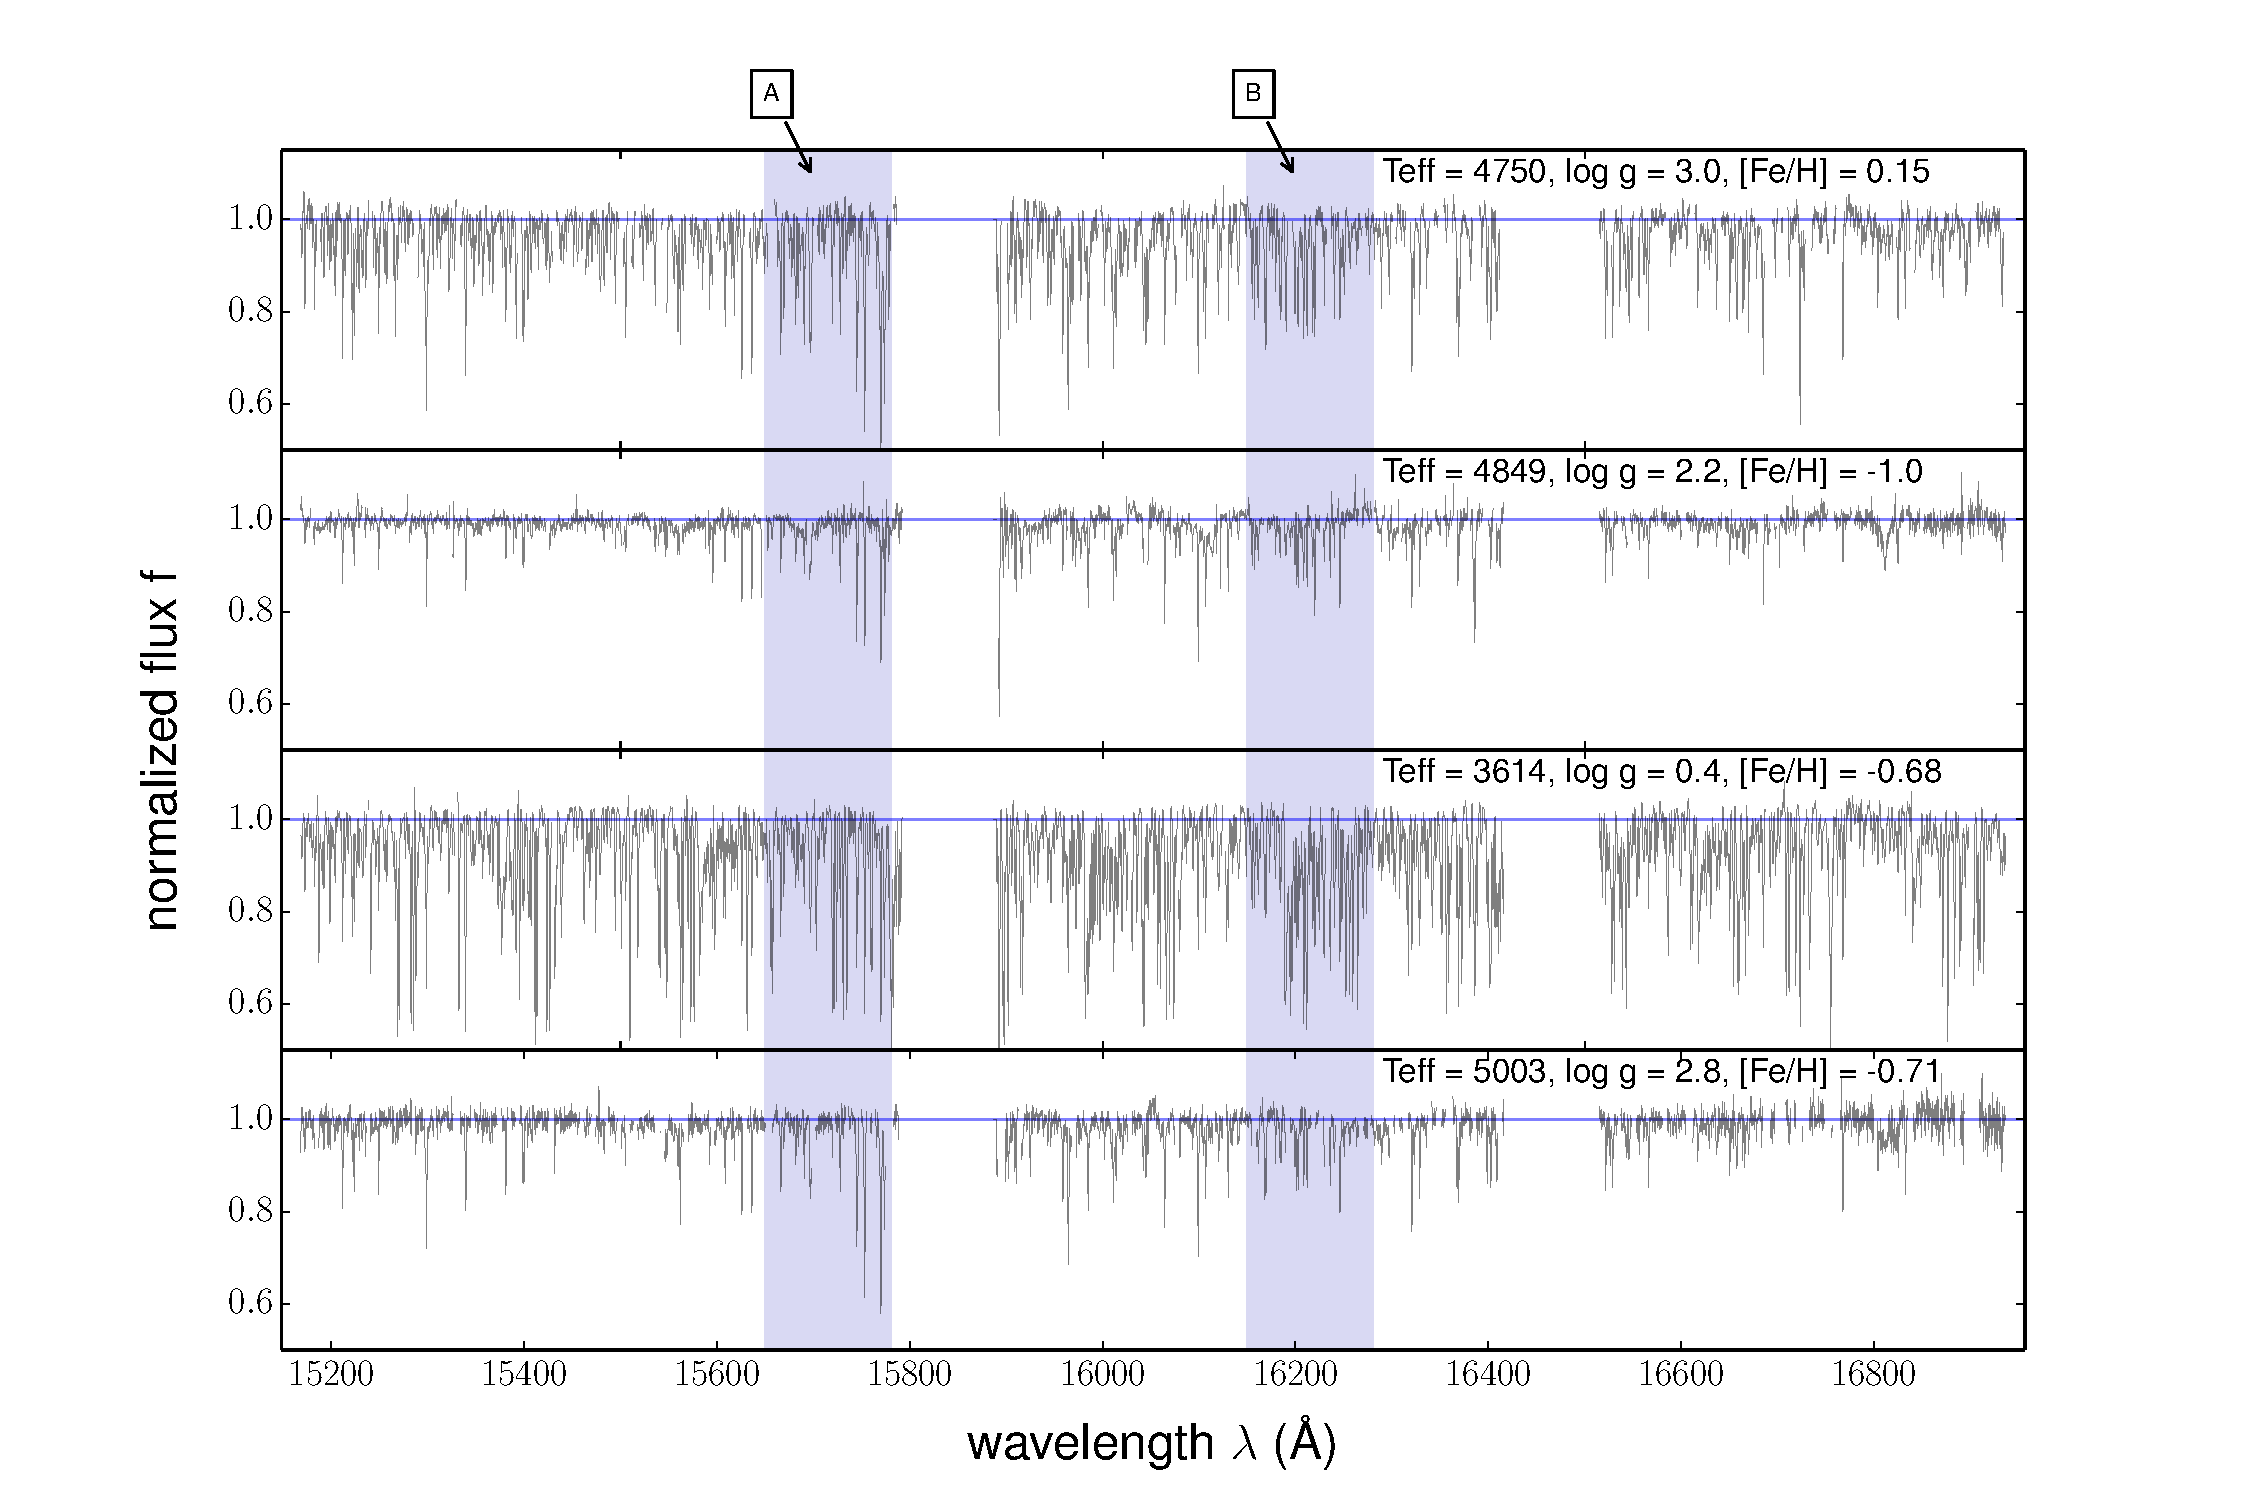
\includegraphics[width=\hsize]{./plots/four_examples3.pdf}
\caption{Continuum normalised spectra for stars across a range of stellar parameters; at top, two stars of similar temperatures at different metallicities and at bottom, two stars of similar metallicities and different temperatures. The grey shaded regions A and B indicate demonstrative sample wavelength regions used for subsequent Figures in the paper.}
\label{fig:norm}
\end{figure}


The inverse variances determined from the error arrays are critical for weighting the test data. 
This is not only for continuum normalisation but for determining the labels, so that bad flux levels due to poor sky subtraction, cosmic rays, reduction induced errors, high persistence and other noise sources are not contributing to the derived labels for the star. 
In addition to the variance arrays, the bad pixel masks are used for the \textit{apStar} files run through \tc\, which further improves the performance of our label-transfer. 
We include the bad pixel masks by setting the variance values to a large value where the data are masked, so the inverse variance and weighing of that pixel becomes $\sim$ 0. 

The resampled, reduced and combined spectra arespectra are available for 49,000 stars in 150 of the 170 DR10 fields in the \aspcapstar\ files. There are a further 4000 stars in 20 fields taken in commissioning which are available in the radial velocity combined but not continuum normalised data format in the \apstar\ files and a further 8000 stars taken during commissioning across different fields. 
The commissioning data, for which the \aspcap-corrected labels are not all provided in the DR10 release, is only available in the radial velocity combined but not continuum normalised data format in the \apstar\ files. 
We run \tc\ through the commissioning data but can not evaluate the fidelity of these results as the line spread function of the commissioning data are different from the main survey and consequently the training dataset of stars. 
Therefore, although we similarly process the \apstar\ spectra, returning the labels for these stars in our online table of DR10 parameters, the reliability of these is uncertain and they are subsequently flagged as commissioning data (see Table 1).

%For the tests on these latter files, the training data input was also taken from the \textit{apStar} and the same continuum normalisation procedure as for the \apogee\ \textit{aspcapstar} pseudo-continuum normalised files was implemented using the 3rd order polynomial weighted fit for each of the three chips, using the pre-defined continuum pixels.

In the following sections we demonstrate that \tc\ reproduces \apogee\ \teff, \logg\ and \feh\ using a number of selected fields across the bulge, disk and halo with very small intrinsic errors which are comparable to \aspcap\ intrinsic errors at lower SNR than minimisation techniques. 
We provide an online table with the full set of parameters for \tc\ run through the \apogee\ DR10 data comprising 59,000 stars in 170 fields \textbf{note to mkn you need to add the commissioning stars to this table}.  
We show all the stars run through \tc\ in the \teff-\logg\ plane and validate our method at low SNR.




\section{Spectral Model}
\label{sec:spectralmodel}

The model is that the observed, continuum-normalized spectrum, at each
wavelength, can be explained as a linear combination of real-valued
``labels'', or a linear combination of functions of those labels.
Here the labels will be stellar parameters like effective temperature $\teff$,
logarithmic surface gravity $\logg$, and metallicity $\feh$.
Additionally, the model is that at each wavelength, the observed
spectrum will deviate from the linear combination by some additive
noise contribution, some of which comes from photon noise and
sky-subtraction noise and other instrumental contributions, and some
of which is an intrinsic scatter, presumed independent at each
wavelength.
The model is built using ``training data'' (with known labels) and then
used to tag (or infer labels for) the ``test data''.

In the training data there are $N$ spectra $n$, each of which has
a continuum-normalized flux measurement $f_{n\lambda}$ at wavelength
$\lambda$. Each of the training spectra $n$ has $K$ labels $\boldsymbol{l_{nk}}$, each of which
is (for now) presumed to have negligible uncertainty and contained within a label vector $\boldsymbol{\ell_n}$.

The general model is:
\begin{eqnarray}
f_{n\lambda} &=&
\boldsymbol{\theta_\lambda}^T \cdot \boldsymbol{\ell_n} + \mbox{noise}
\
\end{eqnarray}

where the flux $f_{n\lambda}$ of each spectra at every pixel is a general function of the labels which predict the spectrum given some noise, where $\boldsymbol{\ell_n}$ is some (possibly complicated) function of the full set of $K$ labels, $\set{l}_n$, which is is a vector or blob of the $K$ labels for spectrum $n$ and $\set{\theta}_\lambda$ is the set of parameters controlling the function $\boldsymbol{\ell_n}$ that determines the flux, at each wavelength.
%%

The simplest spectral model is that in which the function $\boldsymbol{\ell_n}$ is
linear in the labels, so this label vector is described as:
\begin{eqnarray}
\set{\ell_n} =  [1, l_1 - \bar{l}_1, l_2 - \bar{l_2}, l_k - \bar{l_k}, .. ] &\equiv& [l_{n1}, l_{n2}, \cdots, l_{nK}]
\label{eq:linear}
\end{eqnarray}.

The $\mean{l_k}$ are offsets (possibly means of the training data) to keep the model ``pivoting'' around a reasonable point in tag space.


Our general model then becomes
\begin{eqnarray}
f_{n\lambda} &=&
g(\boldsymbol{l_n} |  \boldsymbol{\theta_\lambda}) + \mbox{noise}
\end{eqnarray}

Where the noise is a rms combination of the associated uncertainty variance
$\sigma_{n\lambda}^2$ of each of the pixels of the flux from finite photon counts and instrumental effects and the intrinsic variance or scatter of the model at each wavelength of the fit, $s_\lambda^2$. We assumed that the noise is Gaussian, zero mean, and independent for every measurement and the noise model is $\mbox{noise} = [s_\lambda^2+ \sigma_{n\lambda}^2]\xi_{n\lambda}$, where $\xi_{n\lambda}$ is a Gaussian random number with zero mean and unit
variance.

If there are missing flux values in the training data, these can be
handled by setting variances to something very large (or inverse
variances to something very small).

This model leads to the single-pixel log-likelihood function 
\begin{eqnarray}
\ln p(f_{n\lambda}\given\set{\theta^T}_\lambda, \boldsymbol{\ell_n}, s_\lambda^2) &=&
 -\frac{1}{2}\frac{[f_{n\lambda} - \set{\theta}_\lambda \cdot \set{\ell_n}]^2}{s_\lambda^2 + \sigma_{n\lambda}^2}
\label{eq:like}
\end{eqnarray}


The vector $\set{f}_\lambda$ is the set of spectral flux values for
the $N$ objects all at wavelengths $\lambda$.
We can set the parameters $[\set{\theta}_\lambda,s_\lambda^2]$ either by
optimizing the likelihood (\ref{eq:like}) or by applying priors and
performing some kind of probabilistic inference (with, say, Markov
Chain Monte Carlo techniques).
Here we will optimize for now.

In this \sectionname, we are treating the function parameters
$\set{\theta}_\lambda$ and the scatter $s_\lambda^2$ as free parameters, and the
labels in the label vector $\set{\ell_n}$, $l_{nk}$ as fixed.
The likelihood function (\ref{eq:like}) is presented as being a
function of these free parameters.
In the next \sectionname, the tables will turn, and we will treat the
function parameters $\set{\theta}_\lambda$ and scatter $s_{\lambda}^2$ as fixed and
the labels $l_{nk}$ in the label vector, $\set{\ell_n}$, as parameters.
The difference is that here we are treating the training data as
having perfectly known labels, and later we will be inferring labels for
new spectra.

Then, in training, we determine the coefficients at every wavelength for our model:

\begin{eqnarray}
\set{\theta_\lambda} \leftarrow \substack{\mbox{argmax}\\
{\theta_\lambda}  }
\sum_{n=1}^N \mbox{ln p}(\set{f_\lambda} | {\theta_1,...\theta_\lambda})
\end{eqnarray}

The linear-in-labels form (\ref{eq:linear}) has many useful and
excellent properties.
The first is that optimization of the model, at fixed scatter
$s_\lambda^2$ is a pure linear-algebra operation (weighted least
squares); simultaneous optimization of all the parameters
$[\set{\theta}_\lambda,s_\lambda^2]$ is only nonlinear in the $s_\lambda^2$
parameter.

%
The second is that the tag inference (label-transfer; described in the
next Section) on the test data will have a very simple form.
The third is that the coefficients $\theta_{\lambda 0}$, which are discrete
functions of wavelength $\lambda$, can be seen as an estimate of
the \emph{baseline spectrum} (provided that the offsets $\mean{l_k}$ are
the mean tag values over the $N$ training spectra); and the
coefficients $\theta_{\lambda k}$ can be seen as the mean first derivatives of
the expected spectrum with respect to each of the $k$ labels, estimated
over the range of the training data.

The (perhaps) second-simplest spectral model is that in which the
vector $\set{\ell_n}$ is quadratic in the labels: so this label vector is described as:
\begin{eqnarray}
\set{\ell_n} =  [1, l_1 - \bar{l}_1, l_2 - \bar{l_2}, l_k - \bar{l_k}, (l_1 - \bar{l_1})(l_1 - \bar{l_1}), (l_1 - \bar{l_1})(l_2 - \bar{l_2}), .. ] &\equiv& [l_{n1}, l_{n2}, \cdots, l_{nK}] 
\label{eq:quad}
\end{eqnarray}.

This quadratic-in-labels form (\ref{eq:quad}) is similar to and
different from the linear-in-labels form (\ref{eq:linear}) in a number
of ways.
It is still the case that optimization of the model, at fixed scatter
$s_\lambda^2$ is a pure linear-algebra operation (weighted least
squares).
However, tag inference (described in the next Section) on the test
data will no longer be simple; it will now require non-linear
optimization.

The coefficients $\theta_{\lambda 0}$ can still be seen as an estimate of the
\emph{baseline spectrum} (provided that the offsets $\mean{l_k}$ are the
mean tag values); the first-order coefficients $\theta_{\lambda k}$ can still
be seen as first derivatives of the expected spectrum with respect to
each of the $k$ labels, but now evaluated at the baseline spectrum; the
second-order coefficients $\theta_{\lambda kk'}$ can now be seen as mean
second derivatives of the expected spectrum with respect to pairs of
labels $k$ and $k'$



\section{Label-Transfer to Test data}
\label{sec:paramestimate}

In the previous \sectionname, we built data-driven spectral models
from training data.
These models have the property that, given labels, they can be used to
predict continuum-normalized flux, up to observational and intrinsic
scatter.
In this \sectionname, we are going to solve the inverse problem; we
are going to presume that we have spectra, but we don't have labels.
In this case, we will use inference to obtain labels for the untagged
spectra.
These untagged spectra will be referred to as the ``test data'' in
what follows.

In the test data there will be $M$ spectra $m$, each of which---as in
the training data---has a continuum-normalized flux measurement
$y_{m\lambda}$ at each wavelength $\lambda$, and an
associated observational uncertainty variance $\sigma_{m\lambda}^2$.
Again, if there are missing flux values in the test data, these can be
handled by setting variances to something very large.
The difference between the training data and the test data are that the
test data do not (yet) have known labels $x_{mk}$; we are going to infer
these.

Just as in the previous \sectionname, our model leads to the same likelihood function given in
equation~(\ref{eq:like}), but this time seen as
being functions not of the function parameters $\set{\theta}_\lambda$ and
scatter $s_\lambda^2$ but instead as functions of the \emph{labels}.

Then, in determining labels, we use the coefficients of the flux at every wavelength for a star m: 

\begin{eqnarray}
\set{l_\lambda} \leftarrow \substack{\mbox{argmax}\\
{l_m}  }
\sum_{\lambda=1}^\Lambda \mbox{ln p}(\set{f_\lambda} | {\theta_1,...\theta_\lambda})
\end{eqnarray}

where the likelihood functions are given as a function of labels now,
the sum is now over the full set of wavelengths
$\lambda$, and the vector $\set{f}_\lambda$ is the vector of fluxes from
spectrum $m$ for all wavelengths $\lambda$.
These likelihood functions effectively assume that the function
parameters $\set{\theta}_\lambda$ and scatters $s_\lambda^2$ are all known (from
the training data).
New labels $\l_{mk}$ for object $m$ can be obtained either by maximizing
the likelihood function, or else by applying priors
and performing probabilistic inference.
Here we will optimize for now.

When we use the simple linear-in-labels form (\ref{eq:linear}) for the
mean model $\set{\ell_n}$, the optimization to obtain maximum-likelihood labels
(given parameters $[\set{\theta}_\lambda, s_\lambda^2]$) is simple linear
least-square fitting.
This optimization is obtained by straightforward linear algebra on the
spectral pixels $y_{m\lambda}$, and standard frequentist confidence
intervals can be obtained similarly.

When we use the quadratic-in-labels form (\ref{eq:quad}) for the
mean model $Y()$, there is no simple linear-algebra operation that
optimizes the likelihood. 
Instead an optimisation function is used, the python curve$\_$fit routine, which uses a non-linear least squares fit to fit the function to the data. 

We have described how we construct our model and then apply our model to get labels for new stars. 
We now present in Section\ref{sec:results} the results of implementing our model for all \apogee\ data, where we applied a quadratic model; linear in the coefficients and non-linear in the label-inference.  
For the quadratic model we then show this applied to the DR10 data, including at lower SNR and investigate different input training labels. 



\section{Results}
\label{sec:results}

%\textbf{have written but revisit this: placeholder for MKN:  that commissioning data has different line spread function (LSF) and have run it through but unsure how to evaluate results. The stars do not fall in unphysical places on the isochrone and these commissioning data are indicated in the flag in the table with a C. We do find different parameters compared to \apogee\ for the commissioning data, for the fields where params are available. .Also discuss field 4330 centre field seems to fail for coolest stars for aspcapstar files but is okay if I do the normalisation on the apstar files without pre-continuum normalisation} % - only field where results diverge form apogee though for non-commissioning files, but in sensible place on isochrone.} 

Using only 545 stars as a training dataset, \tc\ successfully reproduces all \aspcap\ DR10 labels and we present five primary results from the implementation of \tc\ through the DR10 \apogee\ dataset. 
The first is the demonstration, via tdhe scatter of the fit, that our model is a good fit to the data. 
This shows that our model is predictive and we perform a cross validation to assess the errors we expect for the test data. 
A cross validation performed with a take-one-cluster out test however tells us that our training data sample is too small, each cluster is critical to the results. 
It is clear from our results that we are also critically lacking in dwarf training data. If the Pleiades stars, which comprise the dwarfs, are removed we can not recover parameters for dwarfs and so can not differentiate dwarfs in the test data.

Via our method, we can use the model for determining continuum pixels, which are robust and true continuum over the label-space of the training data. 
The determination of continuum pixels used in continuum normalisation is a key second result and we implement this for both training and test data and validate it is robust across SNR. 

This success of the method using the DR10 data are our third result. 
Despite the critically constrained training dataset for our model, the label-transfer to the DR10 test data works extremely well.
This showcases the strength in this approach, that with only 545 training stars, we can reproduce all DR10 labels for the stars in the \apogee\ survey, quickly and simply.  
We reproduce the \aspcap\ DR10 labels, of \teff, \logg\ and \feh\ with errors of \teff\ $<$ 100 K, \logg\ $<$ 0.20 dex and \feh\ $<$ 0.10 dex. 
The rms dispersion of \apogee\ -- \tc\ is no larger than \apogee\ parameter errors reported in \citep{Meszaros2013} as our method generates insignificant errors at the SNR of the combined visit \apogee\ data.
We also report results for dwarfs but these are constrained by the very limited dwarf set in our training dataset, and we do not provide a robust measurement of these stars across metallicity, given our single metallicity dwarf training dataset.

The fourth result is that objects which are not in our training dataset have unphysical labels. 
These objects were found to be fast rotators, which can be excluded using the \aspcap\ rotation warning set flag. 
This demonstrates that we can only be as good as our training set. 

The final result that we report is that \tc\ returns robust stellar parameters at an SNR of $<$ 30. 
For this test we do not nosify the spectra but rather use the single visit spectra available in the \textit{apStar} DR10 data files. 
The performance of \tc\ at low SNR reflects both the success of the continuum identification and the advantage in using \textit{all} of the available information in the spectral range to characterise the labels by allowing the regression to determine which pixels control the labels themselves.


\subsection{The model} 

To evaluate the label-transfer method, we performed the simplest implementation of a first-order linear model comprised of four coefficients (Equation \ref{eq:4}). 

\begin{equation}
\ell_n = \theta_0 + \theta_1 \teff\ + \theta_2 \logg + \theta_3 \feh 
 \label{eq:4}
 \end{equation}

The first-order linear model was too inflexible to describe the behaviour of flux with the labels and at the parameter limits of the \feh\ and \logg\ the input training labels could not be returned by the model. 
Different metallicity regimes showed different trends in temperature and \logg\ and the dwarf labels were not well reproduced and dwarfs and giants separated out into different behaviours in the labels. 
This is not surprising given it is known that absorption features and particularly strong lines, do not behave linearly to the first-order, as a function of stellar parameters. 
The linear first-order model can be vastly improved by selecting only weak line regions, and excluding all strong lines by implementing a cut on the normalised flux considered for the coefficients fit in the label-transfer. 
The loss of information in the exclusion of a pixels to compensate for an inflexbile model is however clearly suboptimal. 
An exception where this basic implementation would prove extremely useful is for any front-end to other methodologies of label-determination. 
This most simple version of the regression analysis is extremely fast for determining baseline stellar labels. 
% I am putting this in because at present a lot of surveys use some "fast" method first to get a first pass estimate to input to their pipelines - this might get their attention as this is *a lot* faster than what they are currently doing I believe. 

The second simplest model we can implement is the quadratic model, with ten coefficients, $\theta_{1,2..10}$ describing the labels (\teff, \logg, \feh) (Equation \ref{eq:10}).  
Overall, this model describes the behaviour of the flux with the labels across their label-space fairly well and significantly better than the first-order linear model within the parameter range of these stars. 

\begin{equation}
\begin{split}
\ell_n = \theta_0 + \theta_1 \teff\ + \theta_2 \logg + \theta_3 \feh + \theta_4 \teff^2 + \theta_5 (\teff \logg) + \\
\theta_6 (\teff \feh) + \theta_7 \logg^2 + \theta_8 (\logg \feh) + \theta_9 \feh^2
\end{split}
 \label{eq:10}
 \end{equation}

To assess the uncertainty of our quadratic model implemented in \tc\, we perform a take-one-star out test on the training data. 
This is a conservative way to check our expected error bars on our test data given our model. 
For the take-one-star out test we train the model iteratively on all stars except for one excluded one, and then run the removed star through \tc\, to see how well the model can predict the labels for the removed stars. 

Figure \ref{fig:takeonestarout} shows the cross-validation results for the take-one star out test, comparing the input labels to the output labels, for each of the three labels, for each star. 
The results for the bias and rms are indicative of how well our model performs over the full label range of our data and these variances will inherently include the uncertainties on the input labels (from ASCPAP corrected values, of \teff $<$ 150 K, \logg\ $<$ 0.2 dex and \feh\ $<$ 0.1 dex \citep{Meszaros2013}. 
The precision values are the typical internal errors of the optimisation function to return the respective labels for a given star. 
There are outliers in Figure \ref{fig:takeonestarout}, and certain cluster members of M3 in particular, for example,  are offset in \teff\ and \logg\ space. 
The single dwarf cluster shows the poorest determination in the \feh\ label and this cluster was set at a single metallicity, dissimilarly to the other training data which used \aspcap\ corrected parameters which were provided. 
The rms is comparable to the estimated \apogee\ errors. The take one out test is performed with training data input with \aspcap-corrected labels and the rms error improves by a further 10\% in \teff\ and \logg\  by adopting `isochrone-corrected' labels, obtained by moving the star to the nearest position on the isochrone. 
%Removing this cluster improves the rms in the \teff\ and \logg\ labels by $>$ 10\%

\begin{figure}[h!]
\centering
%  \includegraphics[scale=0.3]{./plots/takeoneout_diag_test18_222.pdf}
    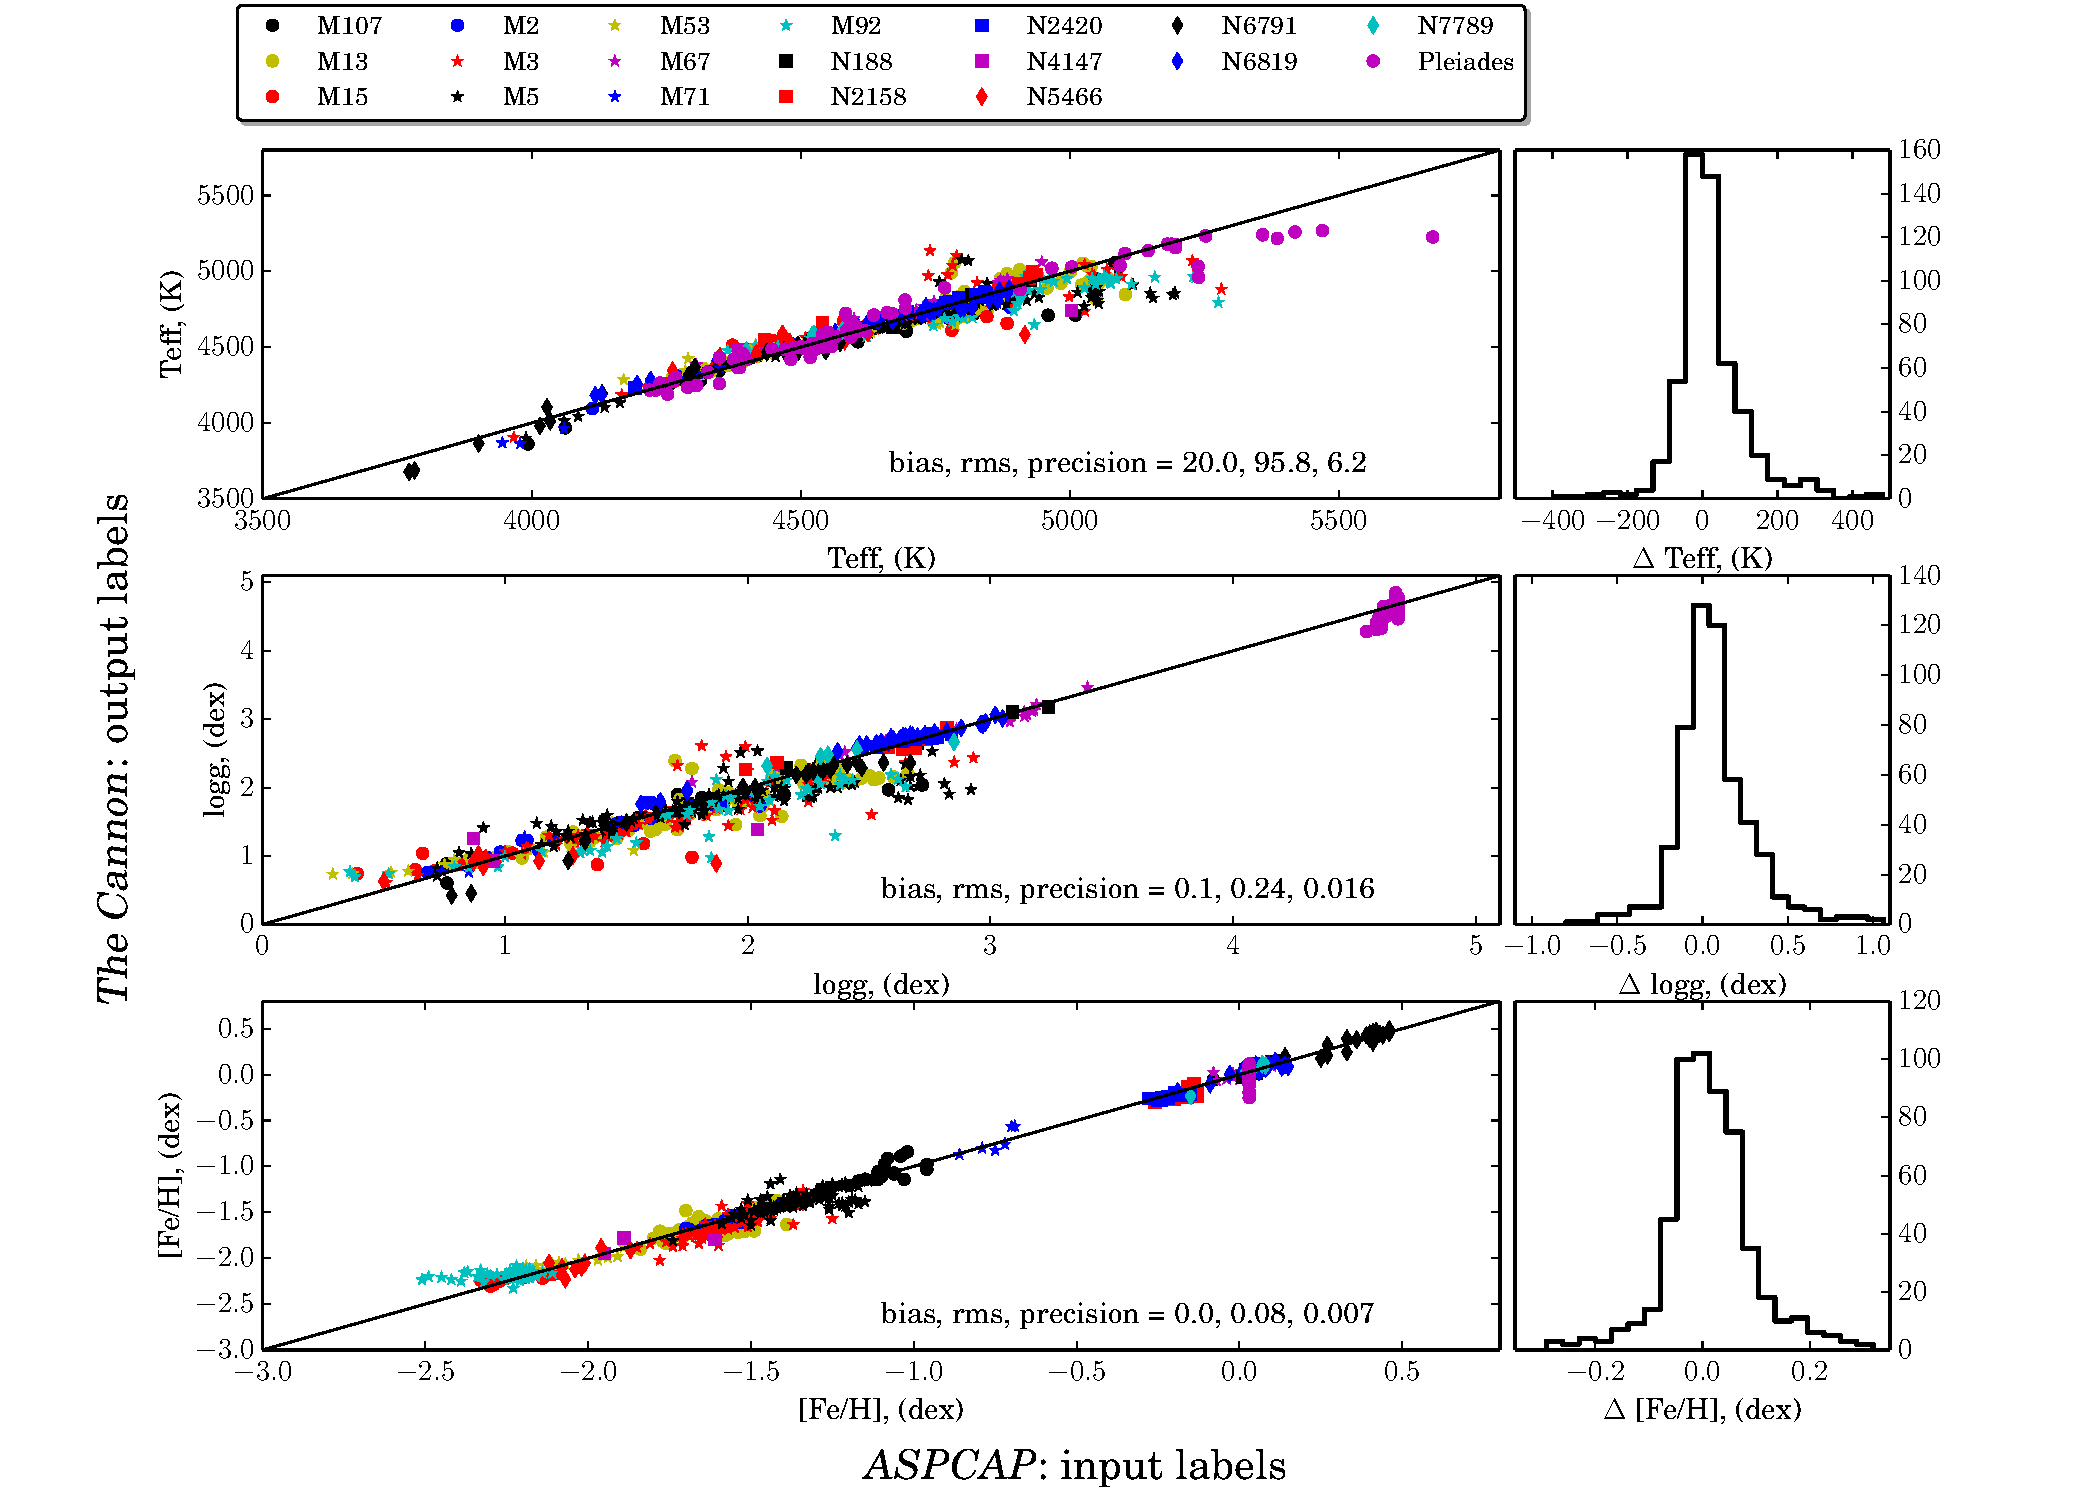
\includegraphics[scale=0.45]{./plots/takeout_hist.pdf}
\caption{The take-one-star-out cross-validation of the 545 stars in the training dataset and corresponding histograms at right, showing \tc\ output -- \apogee\ input labels, where the y axis on the histograms is the number of stars.}
\label{fig:takeonestarout}
\end{figure}

%\begin{figure}[h!]
%\centering
%  \includegraphics[scale=0.45]{./plots/mkn_labels.pdf}
%\caption{Take-one-star-out cross-validation of the 530 stars in the training dataset with own-labels}
%\label{fig:takeonestarout_own}
%\end{figure}

The outlying stars in Figure \ref{fig:takeonestarout} may be due to an anomalous scale of the input labels of these stars compared to the other training data, or it may be a consequence of the model being too inflexible to properly model how flux changes with labels across the parameter space of the training dataset. 
The temperature of the dwarfs is offset low at increasing temperature, compared to the input labels, so the model may be limited in describing the difference between dwarf and giant spectra. 
There is a flattening at the low metallicity end of the model in \feh\ in the output labels at \feh\ $<$ -2.2, however this value of \feh\ = --2.2 also corresponds to the literature value of this cluster, M5 \citep{Meszaros2013}. 
The lower metallicity of the \aspcap\ label may represent internal scatter in the \aspcap\ results.

A take-one-cluster-out test significantly degrades the model, increasing the rms errors to $<$ 150 K in \teff, $<$ 0.4 dex in \logg\ and $<$ 0.12 dex in \feh. 
This indicates that our training set is too small and each cluster is very important to include in the model to return labels for the stars. 
The consequence of removing the Pleaides cluster is that dwarf stars can no longer be differentiated from giants.
 The model can certainly improve and training dataset represents a near minimal subset of stars. 
 Tests including additional labels (e.g. [$\alpha$/Fe]) shows that the rms decreases across all labels with an additional label constraint. 
% and our own label in \logg\ shows an improved performance in the rms for the take-one-star out test shown in Figure \ref{fig:takeonestarout_own}

The results for the first-order coefficients $\theta_{0,1,2,3}$ and the scatter of the fit for the quadratic-in-labels model in Equation \ref{eq:10} is shown in Figure \ref{fig:coeffs} across the narrow regions (A) and (B) of the spectra, marked in Figure 1. 
The top panel shows the zeroth order-coefficient $\theta_0$ or the baseline spectra of the model. 
The mid panel shows the first order coefficients $\theta_{1,2,3}$ in \teff, \logg\ and \feh. 
In the top panel of Figure \ref{fig:coeffs}, the red, blue and green shaded regions show the highest 2$-\sigma$ coefficient values $\theta_{1,2,3}$ in the \feh, \teff\ and \logg\ labels respectively. 
These regions indicate where these flux levels are strongly proportional to these labels and highlights the differences between the labels in their flux dependancy. Note there are many regions where the \feh\ label dominates in contribution to the flux. 
For the first label profiles for example in the middle panel of Figure \ref{fig:coeffs}, there is typically asymmetry for a given absorption feature, in the flux and the labels. There are very few regions where the flux is a function of only one of the labels, and pixels are typically covariant (that is, the same pixel will have a higher flux at both lower \teff\ and higher \feh).
 The strongest \logg\ dependence is typically associated with weak lines including the wings of the feature and the \feh\ label, with strong lines, particularly the depth of the line. 

From the bottom panel of Figure \ref{fig:coeffs}, it is clear that there is significant covariance between the labels. 
The bottom panel shows the scatter of the fit, indicating the dispersion of the flux of the training data around the model at each pixel. 
The scatter is small and this indicates that our model is a good representation of the data. 
However, the scatter is highest where the most information in the spectra are contained. 
This indicates that either our model is restricted or the labels of our training dataset are imperfect, or both. 
From this baseline flux, the continuum pixels have been determined, and these are marked in the black dots in the top panel of the Figure. 
These continuum pixels are used for the final continuum normalisation for the stars, both training data and test data. 

% and the mid-panel corresponds to the intersect of the model of the training sample, with regions of first order label dependence shaded in the different colours corresponding to \teff, \logg\ and \feh.

By returning coefficients, we have a tool which \textit{describes the flux in a quantitative way as a function of stellar labels}, thus removing degeneracies and improving the prospects for determining stellar parameters, by modelling covariance rather than attempting to minimise it. Regions that have dependencies on only one of the labels can also be easily identified. 

  %made with run -i makeplot_scatter_test18_step.py
\begin{figure}[h!]
\centering
    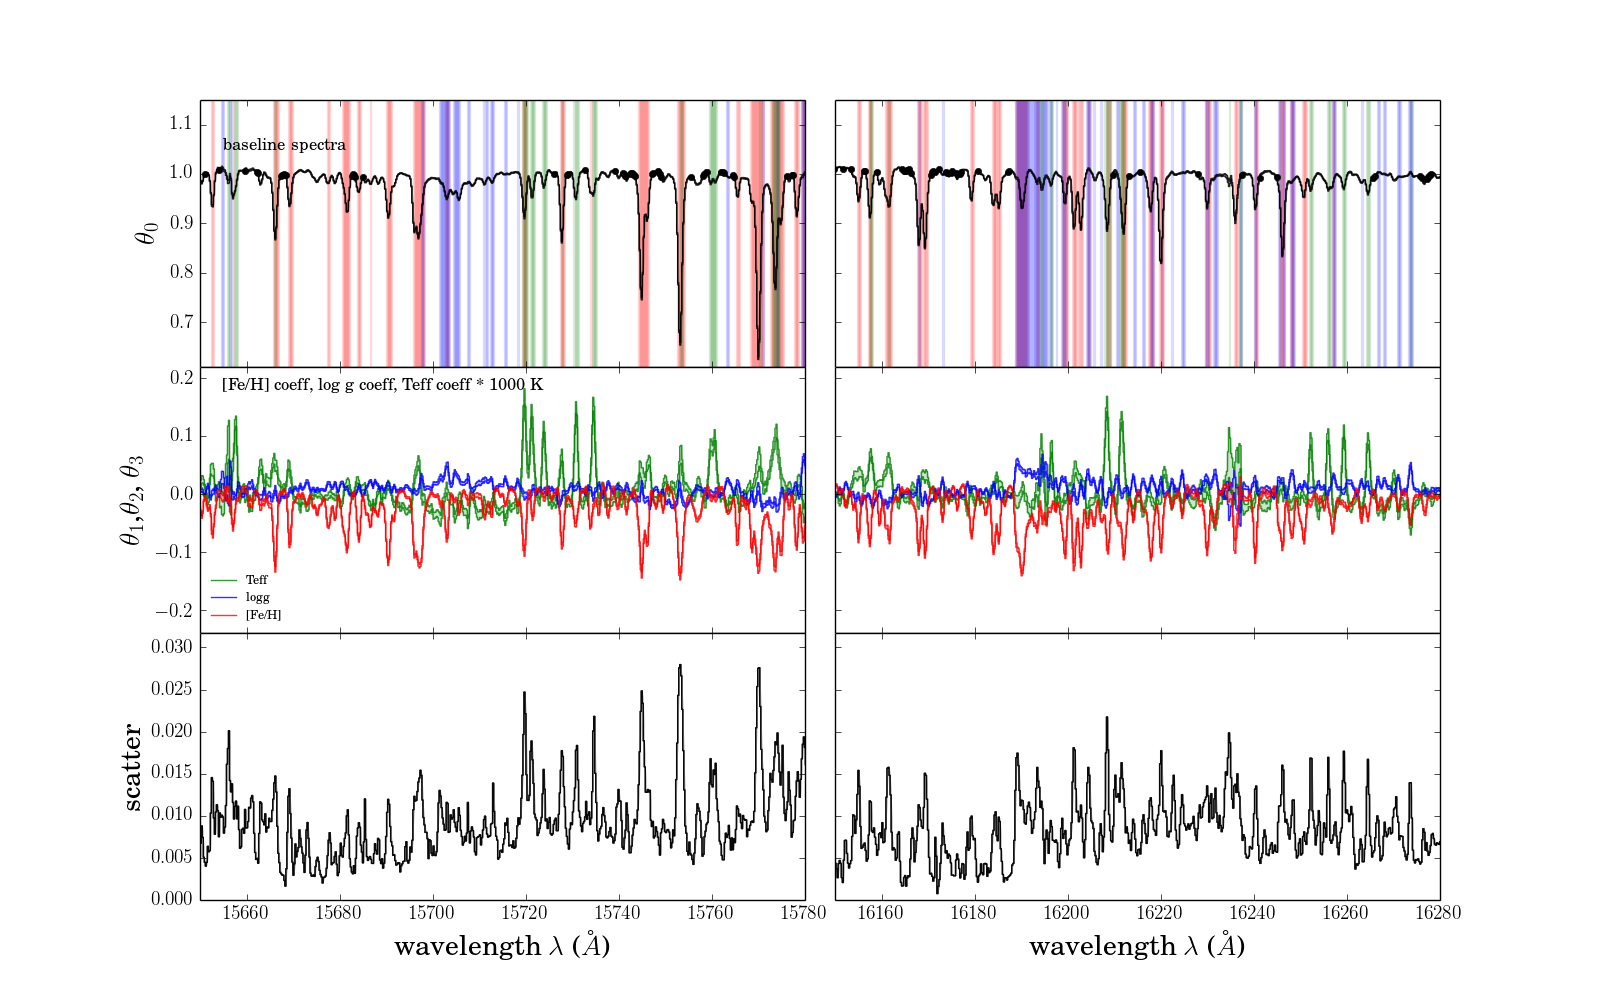
\includegraphics[width=\hsize]{./plots/R1_continuum4.png}
  \caption{The first order coefficients and scatter across the sample regions of the spectra from Figure 1, A and B. Top panel: the baseline spectra from the first coefficient from the training dataset; mid-panel; the first three coefficients ($\theta_1$, $\theta_2$, $\theta_3$),  which correspond to the first-order label terms ($\teff, \log, \feh$); bottom panel: the scatter of the fit.  The red, blue and green shaded regions in the top panel show the highest 2$-\sigma$ coefficient values in the \feh, \teff\ and \logg\ labels respectively. This indicates where these flux levels are strongly proportional to the labels. Note the \feh\ label is dominant in the contribution level and from the bottom panel it is clear that there is significant covariance between the labels and lesser regions of strong \logg\ dependence, across these sample wavelength intervals.}
\label{fig:coeffs}
\end{figure}
\textbf{We had once talked about scaling these coefficients - how do I do this exactly - x mean/range?}




\textbf{DWH: caveat about our cross-validation and signal to noise}. 

\subsection{Continuum identification}

The continuum pixels, which are shown in Figure \ref{fig:coeffs} for wavelength regions A and B,  have been determined from the quadratic model using a combination of the flux level and the coefficients returned.  From the baseline, or zeroth coefficient of the flux returned in the first coefficient, 35\% of the pixels across this wavelength region have a pixel level within 1\% of flux = 1. However, regions where the intersect-flux is $\sim$ 1 are not representative of continuum for all stars in the training set, e.g. metal rich stars. It is insufficient to select pixels that are simply near the intersect-flux in isolating continuum regions. Instead, we are informed by the coefficients of the fit. A set of coefficients which are near 0, is indicative of a pixel region where there is no dependence, or negligible dependence of the flux on the labels, across all of the training spectra. We make a continuum selection taking the 15\% of pixels with coefficients nearest 0 for each coefficient and a flux selection of 1 $\pm$ 0.15. This criteria returns around  7\% of pixels, which we adopt as true continuum pixels for data that spans the parameter range of the training set. We use the inverse variance weighting of these pixels for the corresponding Chebyshev polynomial fit which we find to provide a robust continuum normalisation across the stars that are within the parameter range of the training set, across all SNR. 

\subsection{DR10 Comparison}

Although our model is sub-optimal in its size and its diversity of spectra, we are nevertheless able to reproduce all of the \aspcap\ labels for (non-comissioning) DR10 spectra. We have run \tc\ through all 47,000 stars in 150 fields in DR10 contained in the available \textit{aspcapstar} files as well as an additional 4800 stars in 20 commissioning fields for which no \aspcap\ parameters were provided in DR10, made available in the (non pseudo-continuum normalised) \textit{apStar} files. We also have run \tc\ through the additional commissioning stars available in the \apstar\ files across the fields and in total this comprises 59,000 DR10 stars in 170 fields. %These 170 fields comprise a total of $\sim$ 51,600 \apogee\ DR10 stars. 

The results of \tc\ for all DR10 stars for which we return parameters are provided online in Table \ref{tab:online}. For the 30,500 stars with parameters provided by DR10, we find we reproduce the \apogee\ labels as follows: \teff\ = +12 K $\pm$ 87 K ,  \logg\ = --0.04 dex $\pm$  0.18 dex and \feh\ = +0.01 $\pm$ 0.10 dex in \feh. The rms errors are comparable to the error estimates for \apogee\ parameters in \citet{Meszaros2013} of $\delta$(\teff) $<$ 150 K, $\delta$(\logg) $<$  0.2 dex and $\delta$(\feh) $<$  0.1 dex in.  The typical internal precision on the measured parameters from \tc\ is  $\delta$(\teff) $<$ 5.6 K in ,  $\delta$(\teff) $<$ 0.01 dex in \logg\ and  $\delta$(\teff) $<$ 0.006 dex in \feh.


\begin{table*}[!h]
\small{
\centering
\caption{Excerpt from full online version of table of parameters for the 59,000 stars released in 170 fields from \apogee\'s data release DR10. Stars with rotation warning = 1 flag set have unphysical stellar parameters and commissioning stars are marked with ``C'', the fidelity of the commissioning stars is uncertain given their different LSF from survey test and training data.} \begin{tabular}{| c | c | c |  c | c | c |  c | c | c |} %51,500
\hline
star ID & \teff\ & \logg\ & \feh\ & $\sigma$(\teff) & $\sigma$(\logg) & $\sigma$(\feh) & $\chi^2$ & \tiny{ROT WARN}\\
{2MASS} &  K &  dex  & dex & K & dex & dex & & \\    
\hline
%21353892+4229507 & 4131.7 &  1.51 & 0.04 & 3.25 & 0.0116 &  0.0042 & 11.06 &  0.0\\
21354474+4250256 & 5028.5 & 4.53 & 0.13 & 9.14 & 0.01 & 0.006 & 3.14 & 0\\
21354775+4233120 & 4730.9 & 2.8 & 0.06 & 12.02 & 0.04 & 0.011 & 1.34 & 0\\
21355458+4222326 & 4780.1 & 2.42 & --0.36 & 8.34 & 0.03 & 0.007 & 2.41 & 0\\
21360285+4231145 &  4552.4 &  1.96 & --0.46  & 10.83 & 0.04 & 0.011 &  1.42 &  0\\
 \hline
\end{tabular}
\label{tab:online} }
\end{table*}  
 

The comparison of \tc\, showing the bias, rms and precision for 6 sample fields, with bulge, disk and halo targeting are provided in Figure \ref{fig:cal}. As for all stars in the survey with \aspcap\ labels, these fields show that we reproduce the \aspcap\ corrected stellar parameters with typical rms uncertainties of \teff\ $<$ 100 K, \logg\ $<$ 0.20 dex and $<$ \feh\ $<$ 0.10. These errors are slightly better than the expectations provided with our cross-validation leave-one-star-out test which may be because the median of the test data stellar parameters are near the median labels of the training data and not concentrated to the extreme ends of the range, which have a higher weighting in evaluating the test data with cross validation. In addition, we also return a fraction of about 15\% dwarfs (not shown in these Figures as \apogee\ does not report ASCAP corrected dwarf parameters for DR10). We exclude the rapid rotators using the \aspcap\ \rotwarn\ flag as we can not return parameters for spectral types not included in our training set. 

In Figure \ref{fig:cal} we show the residuals of \tc\ $-$ \aspcap\ for the 1400 stars from the 6 sample fields as a function of \aspcap\ \teff, \logg\ and \feh. There are weak trends; at low \teff\ $\sim$ 3700 K, we find temperatures about 100 K cooler than \apogee\, at low \logg\ we find $\sim$ 0.15 dex larger \logg\ than \apogee\ and at the lowest metallicities \feh\ $<$ --2.0, we typically report higher metallicities on the order of 0.05 to 0.3 dex. 


%makeplot_fits_v19_bw.py
\begin{figure}[!h]
\centering
  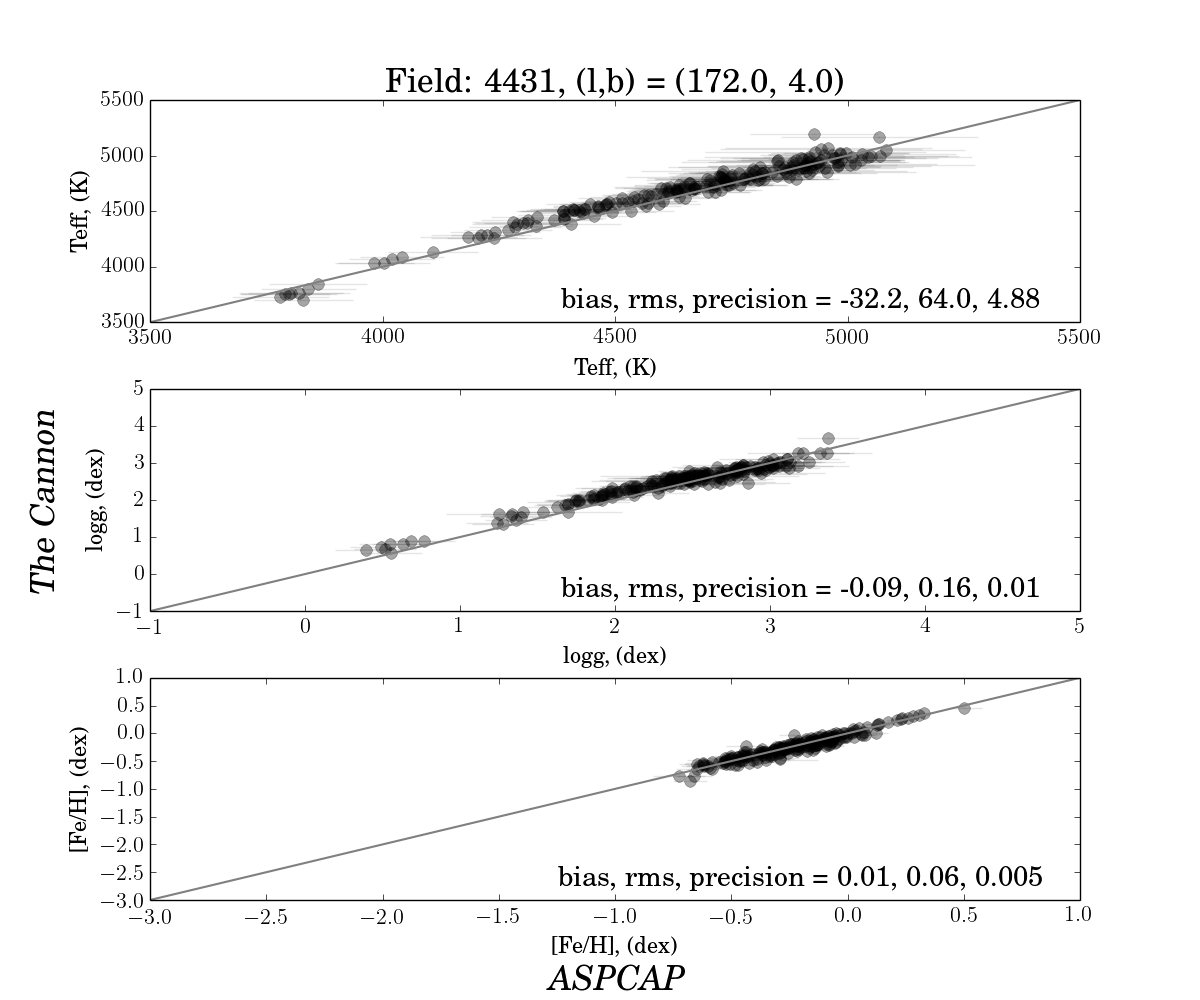
\includegraphics[scale=0.23]{./plots/4431_v19.png}
    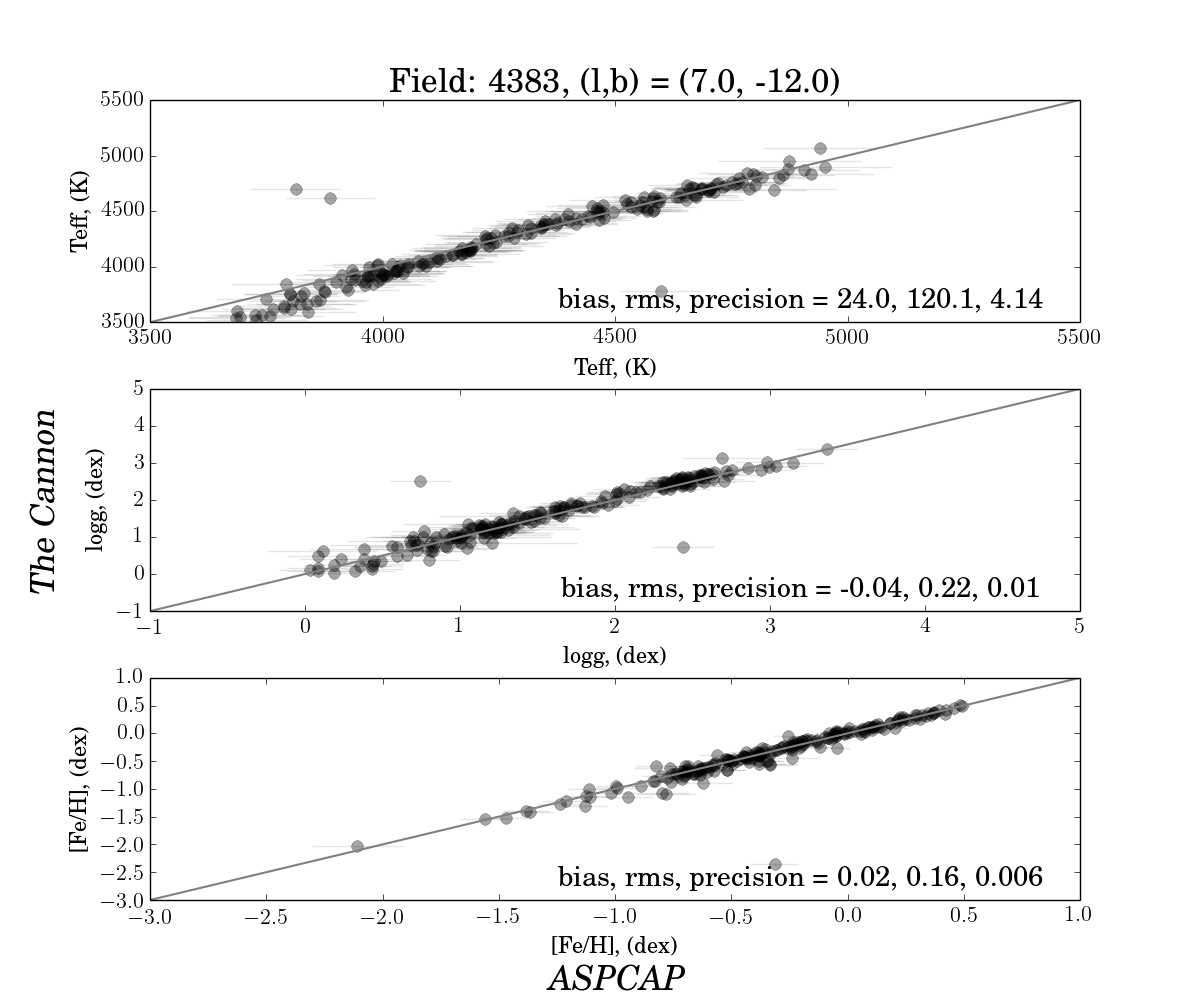
\includegraphics[scale=0.23]{./plots/4383_v19.png} \\
      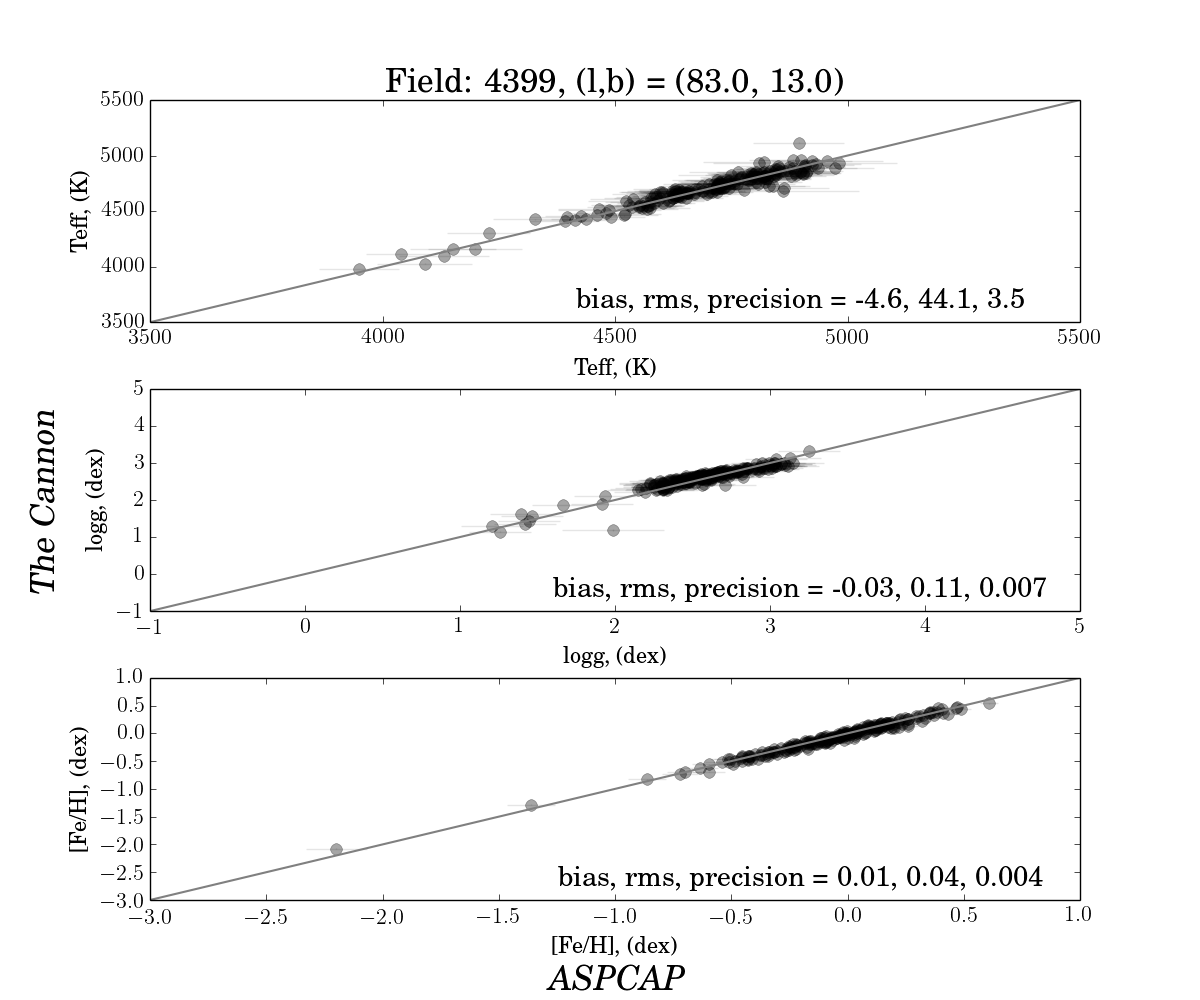
\includegraphics[scale=0.23]{./plots/4399_v19.png}
        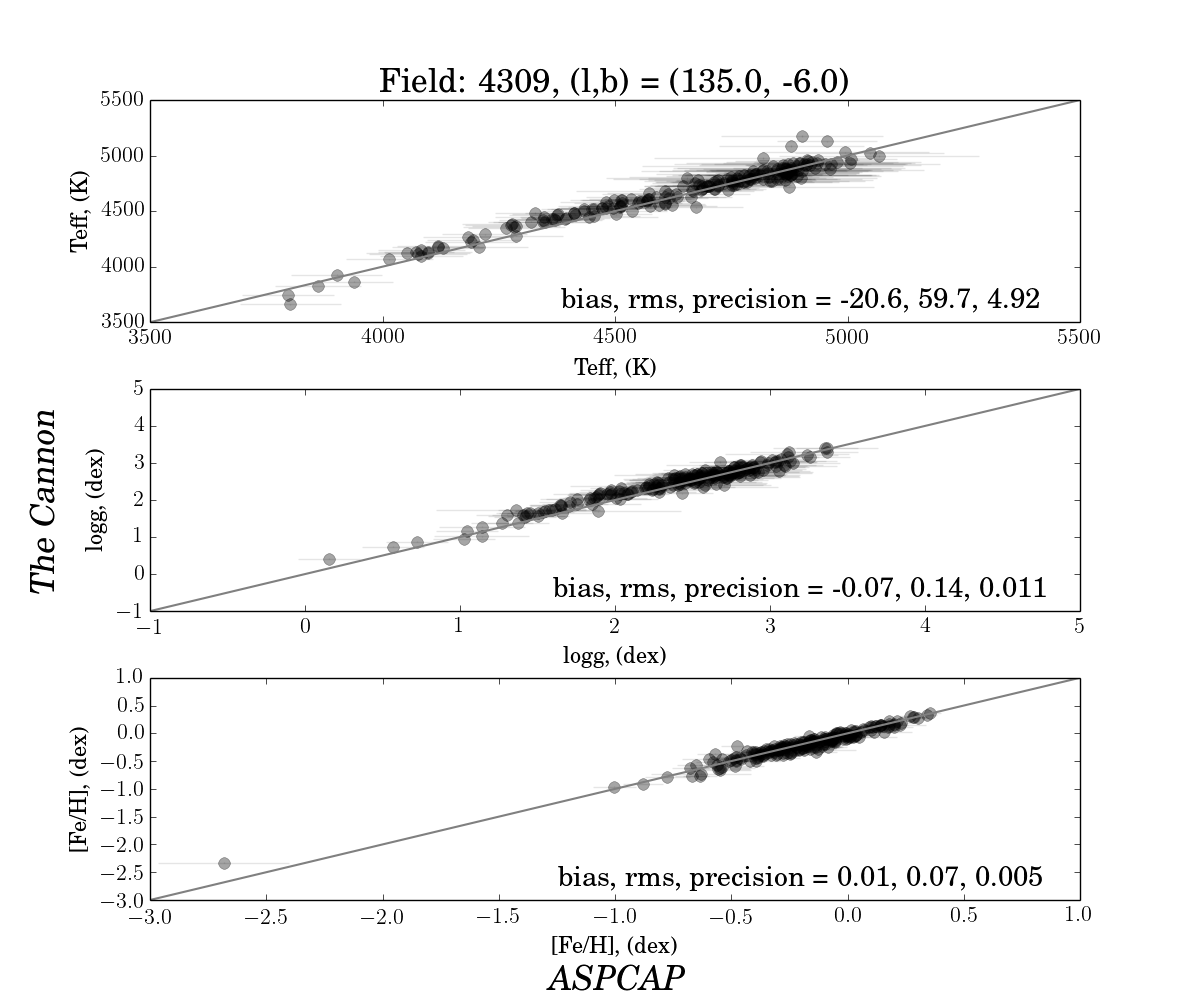
\includegraphics[scale=0.23]{./plots/4309_v19.png} \\
              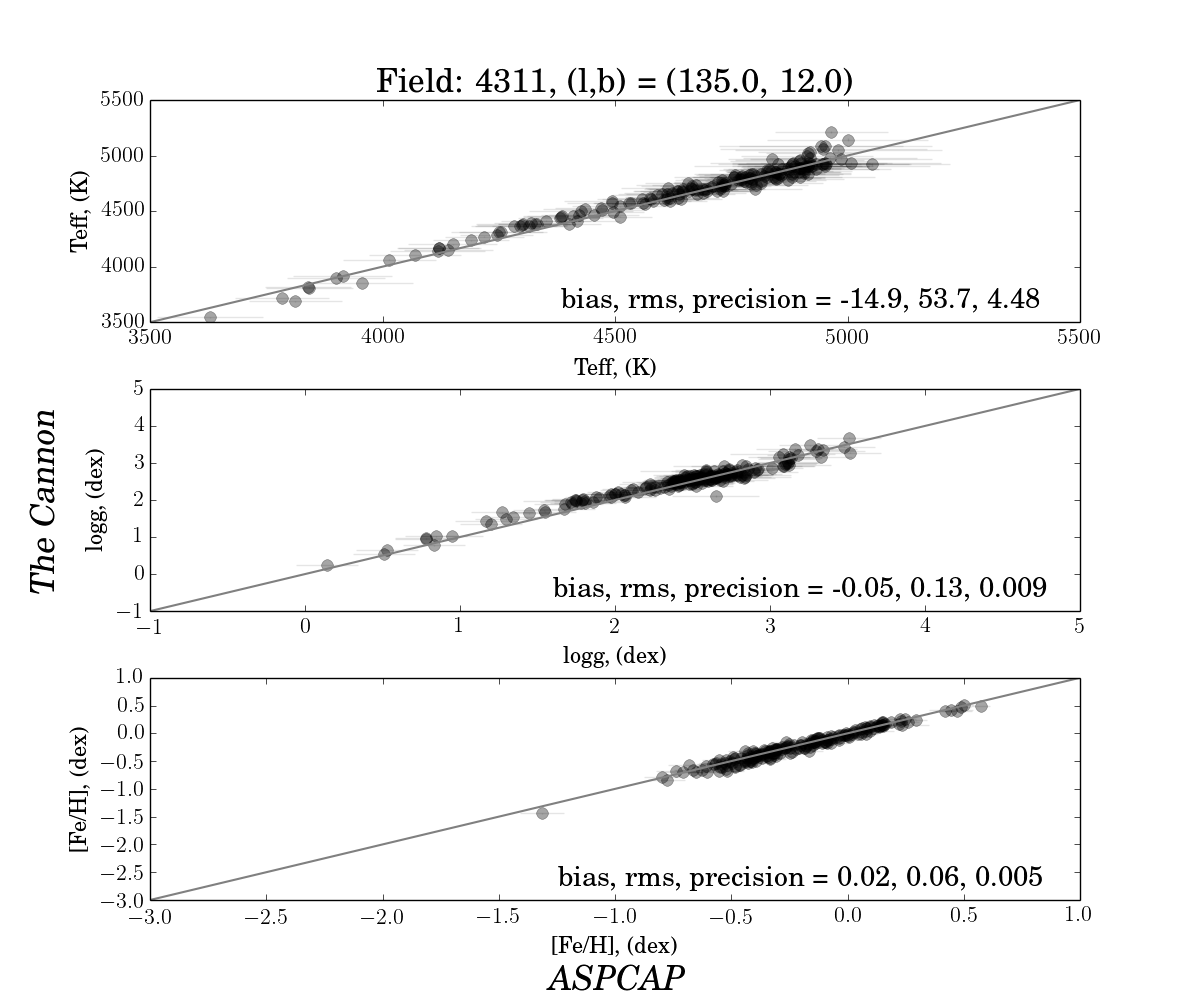
\includegraphics[scale=0.23]{./plots/4311_v19.png}
        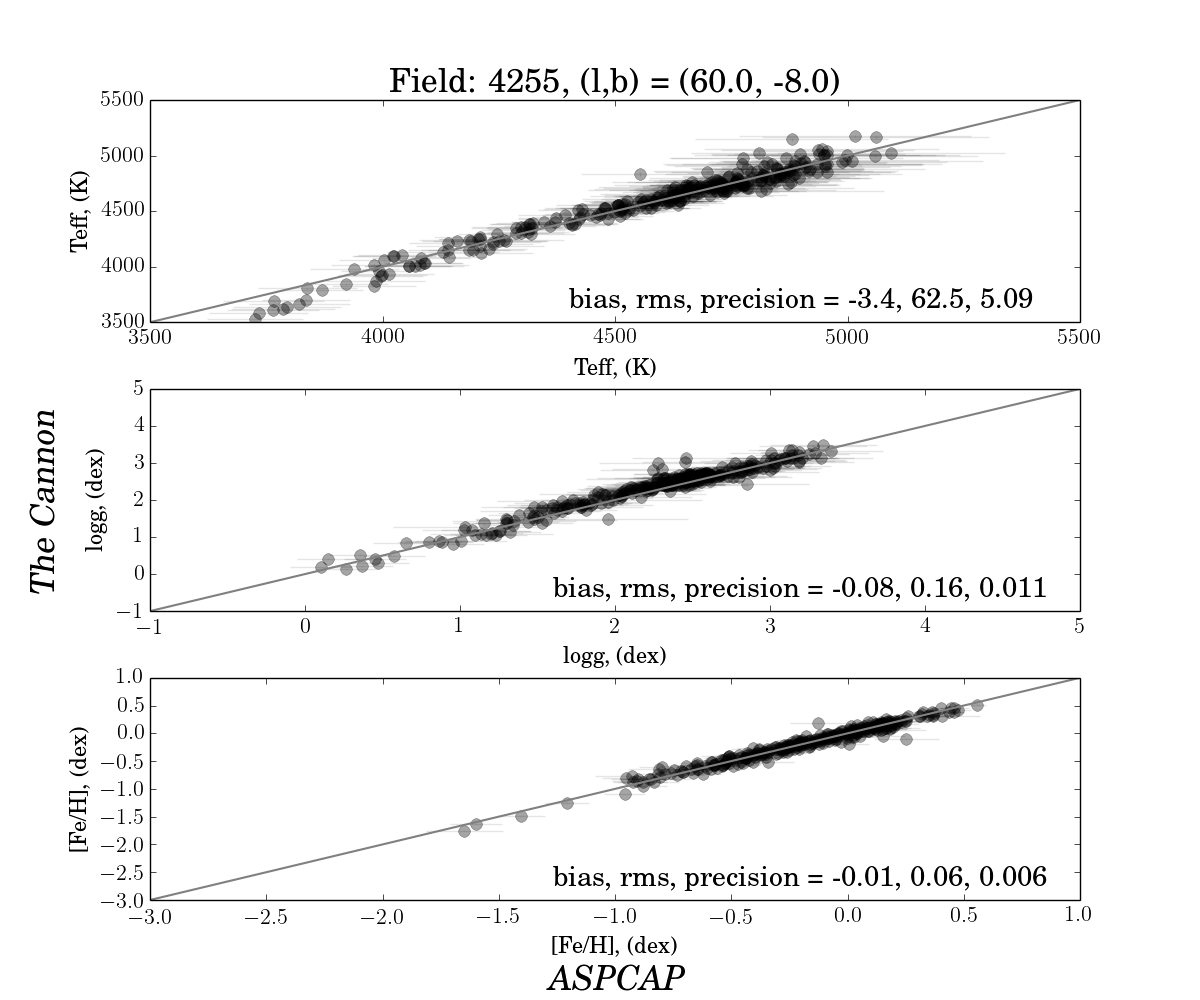
\includegraphics[scale=0.23]{./plots/4255_v19.png} 
\caption{\small{\aspcap\ DR10 versus \tc\ for six different fields including in the disk, bulge and halo. The number of stars is, for each subfigure is 211 (4431), 207 (4384), 217 (4399), 210 (4309), 198 (4311) 319 (4255) }}
\label{fig:cal}
\end{figure}

%run -i makeplot_fits_v19_3by3c.py with plotfits_v19('listin.txt')
\begin{figure}[!h]
\centering
        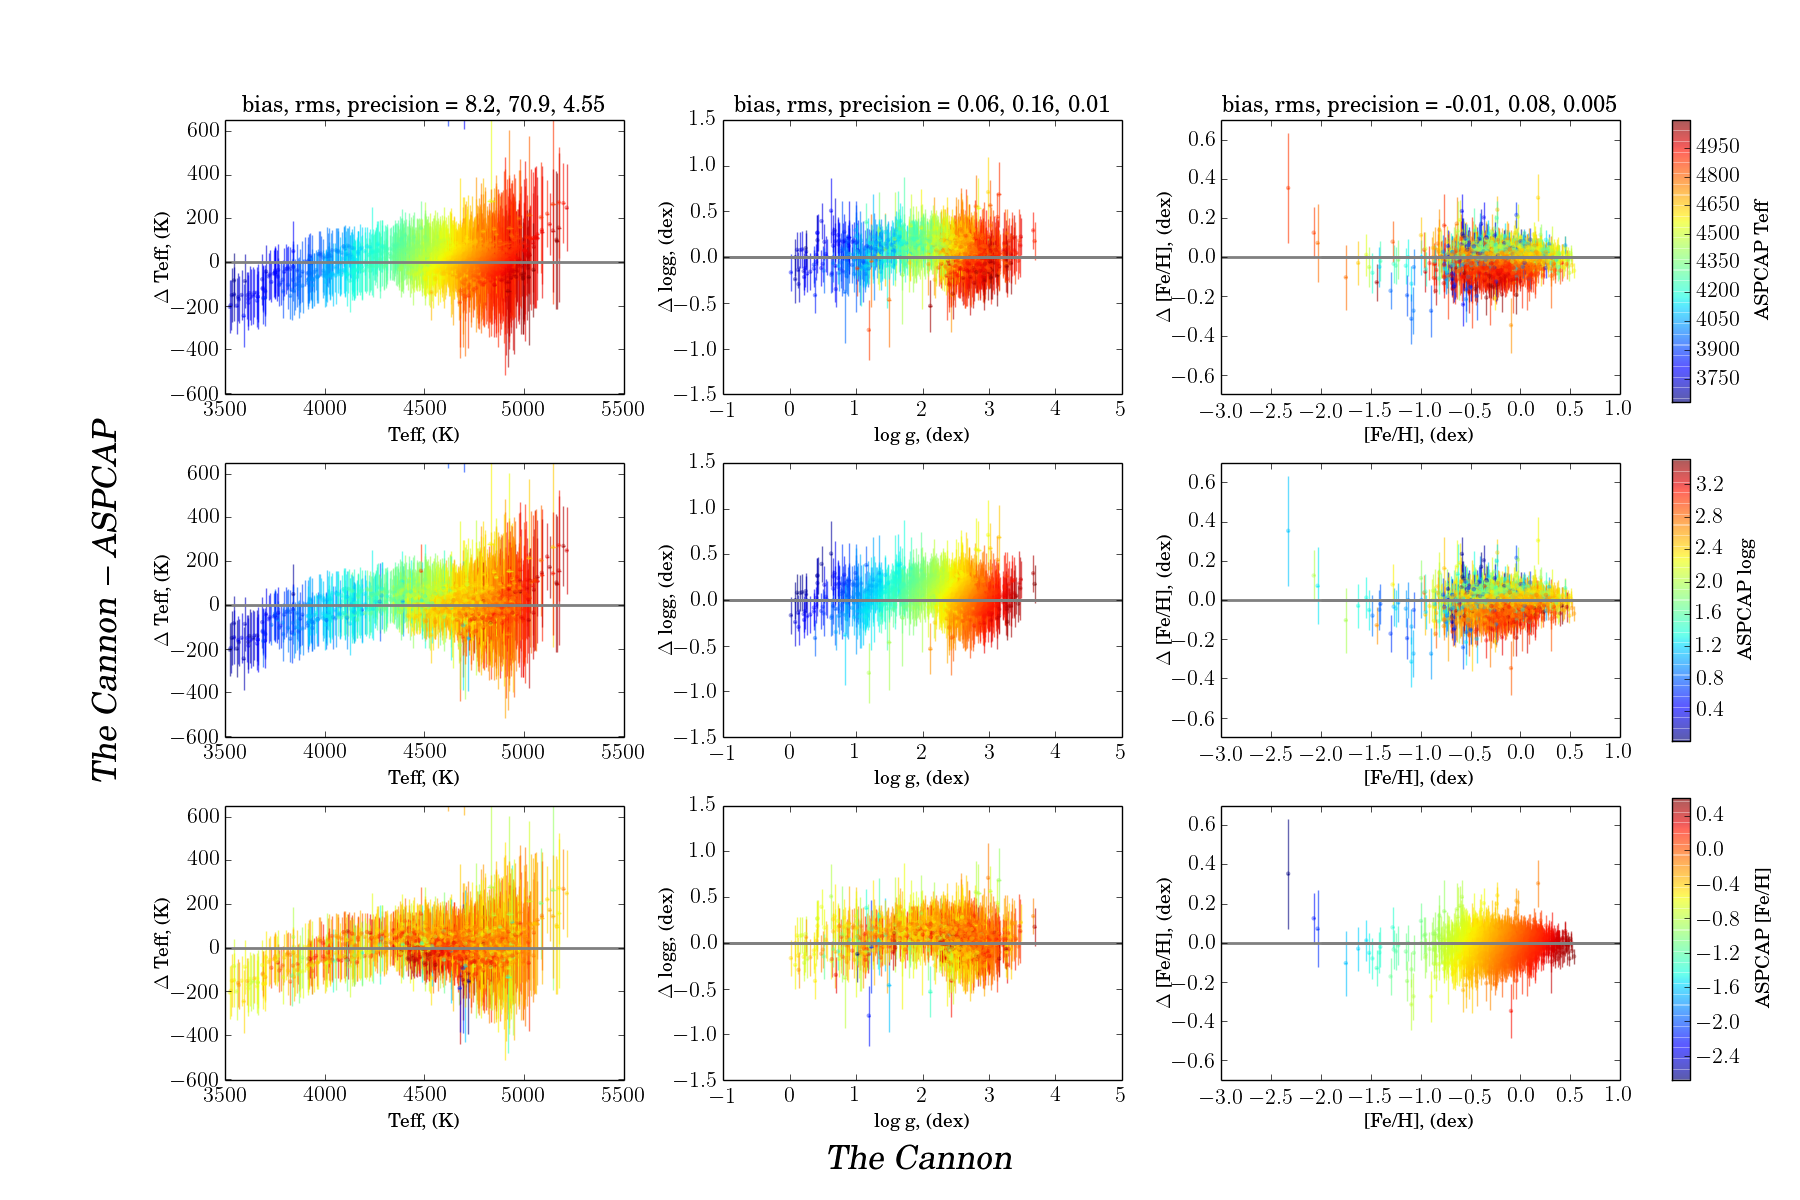
\includegraphics[scale=0.35]{./plots/cplot2.png} 
\caption{The \teff, \logg, and \feh\ trends for the 1400 stars shown in six different fields in Figure \ref{fig:cal}. There are slight trends at the extreme ends of the range in parameters.}
\label{fig:cplot}
\end{figure}


We show the location of the stars in the \teff-\logg\ plane from \tc\ for the stars in DR10 in Figure \ref{fig:iso} where Figure \ref{fig:iso} shows the training labels input directly from \aspcap\ corrected labels and \ref{fig:iso2} shows the results for the isochrone-corrected labels. There are 37,500 stars in these Figures which are remain after excluding stars with the \rotwarn\ flag set, with velocity scatter $>$ 10 \kms\ and telluric calibration target set. For approximately 15\% of these stars, we return dwarf parameters for, with \logg $>$ 4 dex.  The stars that have been determined using targeting flags and inspection of the spectra, to be dwarfs with rotation, lie in an unphysical space at very low \feh\ and log g and have been removed using the \aspcap\ rotation warning set flag. 

Although we find excellent agreement between \tc\ and \aspcap\ by adopting ASCPAP corrected labels and additionally are able to derive parameters for dwarf stars in DR10, the \teff-\logg\ plane for these stars shows an unphysically narrow giant branch  (see the right panel of Figure \ref{fig:iso}). The narrowness of the giant branch is a consequence of the input labels of the training spectra. The results using our isochrone-corrected \logg\ training labels calibration (described in the Introduction) deviate slightly   from the \aspcap\ scale in each of the parameters. However, with these new \logg\ labels, we find a broad giant branch width that is consistent with expectations in \teff-\logg\ space given the metallicity of these stars (see the right hand panel of Figure \ref{fig:iso2}). 

There are not priors to place the stars on any position on the isochrone and that almost all stars lie in physical spaces on the isochrones as shown in Figures \ref{fig:iso1} and \ref{fig:iso2} validates the labels. The labels for the dwarfs are however ill determined, given the single dwarf training cluster and there is a handful of stars at low \feh\ and low \logg\ that do not lie on the isochrone. At metallicities \feh\ $<$ --0.25 the red clump is offset low in \logg. \citet{bovy2014} estimates the consequence of the offset is to shift the red clump and red giant branches 0.2 dex closer together. Our \logg\ labels in Figure \ref{fig:iso} are essentially \apogee\ labels (offset -0.04 dex in \logg\ for DR10) and the left panels show that the red clump branch is offset to higher \logg\ than the red clump branch of the Padova isochrone, for stars \feh\ $<$ --0.25. This offset is on the order of 0.2 dex at \feh\ = -0.5 and is present for both \aspcap-corrected  labels and isochrone-corrected labels. This may indicate that the \aspcap\ temperature scale is offset too cool in DR10 (but as a function of \feh).

%\textbf{have written -find it odd this is not discussed in Jo Bovy's paper: note to MKN: Discuss that red clump is not where it should be for stars $<$ --0.25, Jo Bovy didn't show this in the paper but does mention there is a systematic offset - it's pretty bad though - instead shows apocask stars on the padova isochorne fit. This plot/discussion never appears in apogee papers - is it just as one wants to project the positive aspects and not all aspects of the results that this has been omitted or am i just missing a of it elsewhere?}.

% made with makeonisochrone_v18_bw.py
\begin{figure}[!h]
\centering
  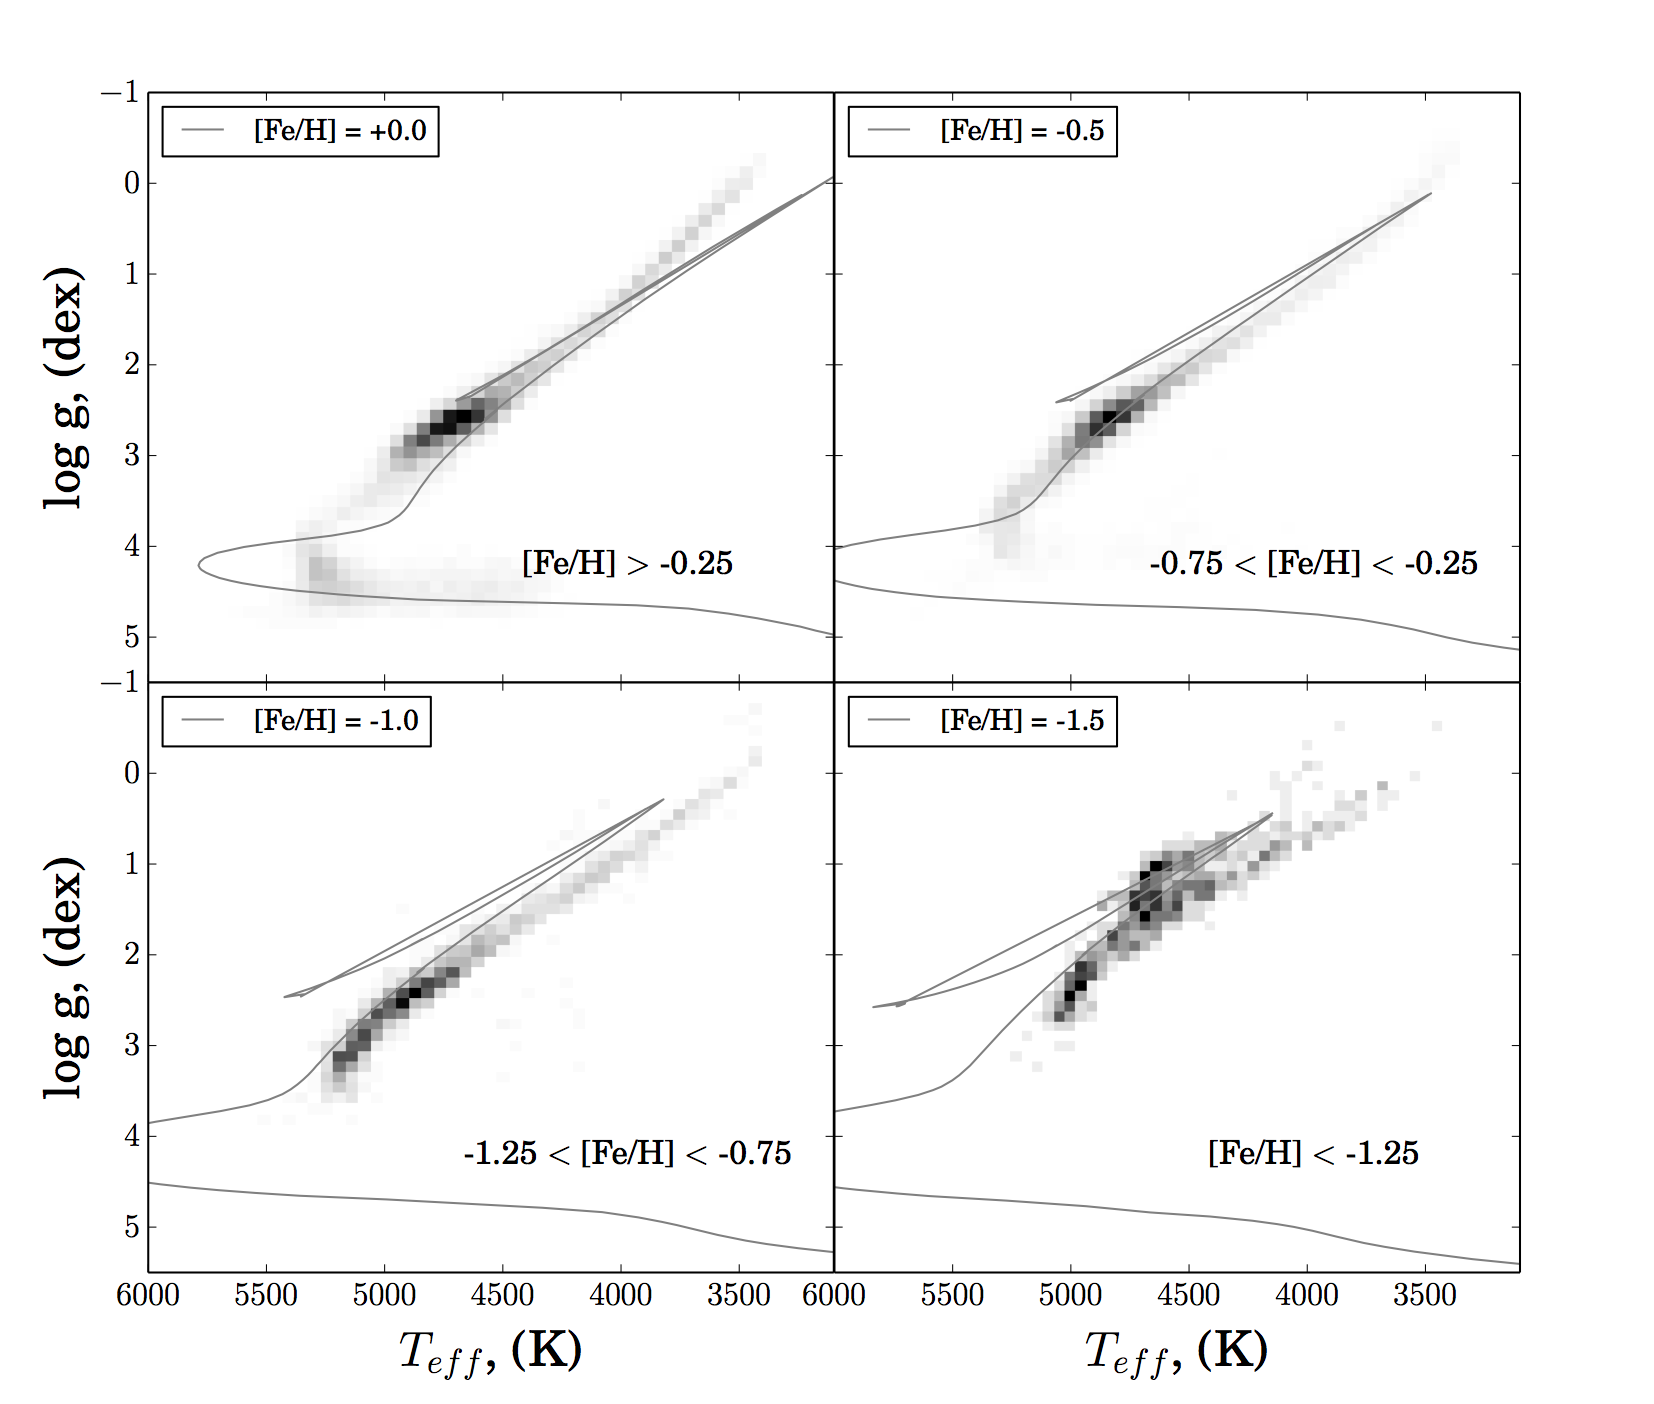
\includegraphics[scale=0.25]{./plots/iso1.png}
  \hspace{-20pt}
    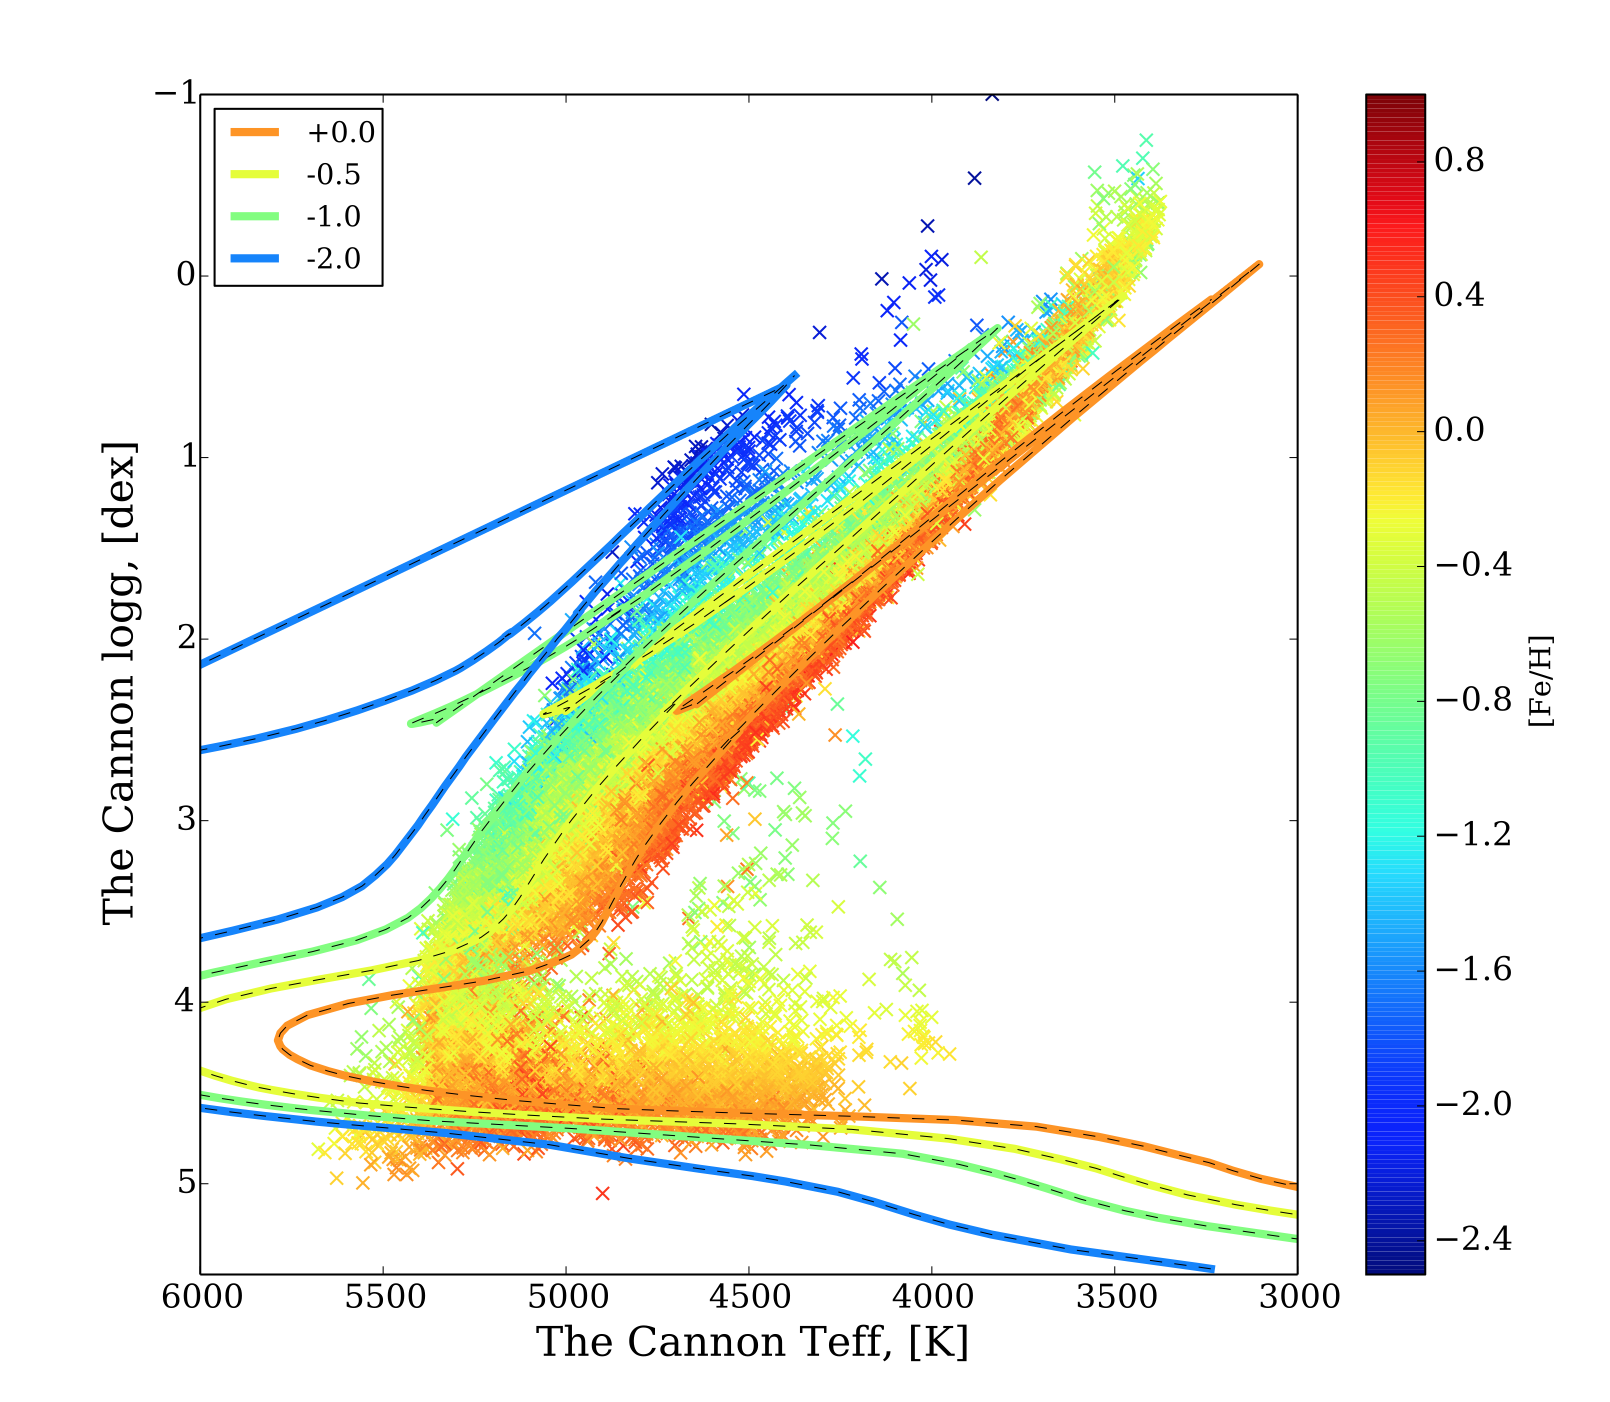
\includegraphics[scale=0.25]{./plots/iso1a.png}
%    \includegraphics[scale=0.33]{./plots/isochrone_mkn20b2.pdf}
\caption{The $\sim$ 38,000 stars from DR10 with \aspcap-corrected training labels, at left shown in four metallicity bins. There are $\sim$ 21,600, 14,000, 1700, and 900 stars in the most metal-rich to metal-poor metallicity bins, respectively. The panel on the right shows all stars coloured in [Fe/H] on the four isochrones. Note the \logg\ distribution at low \logg\ is narrow and offset from the giant branch. The isochrones plotted are 10 Gyr Padova isochrones at the metallicities marked in the upper left hand corners of each sub-panel.}
\label{fig:iso}
\end{figure}


\begin{figure}[!h]
\centering

      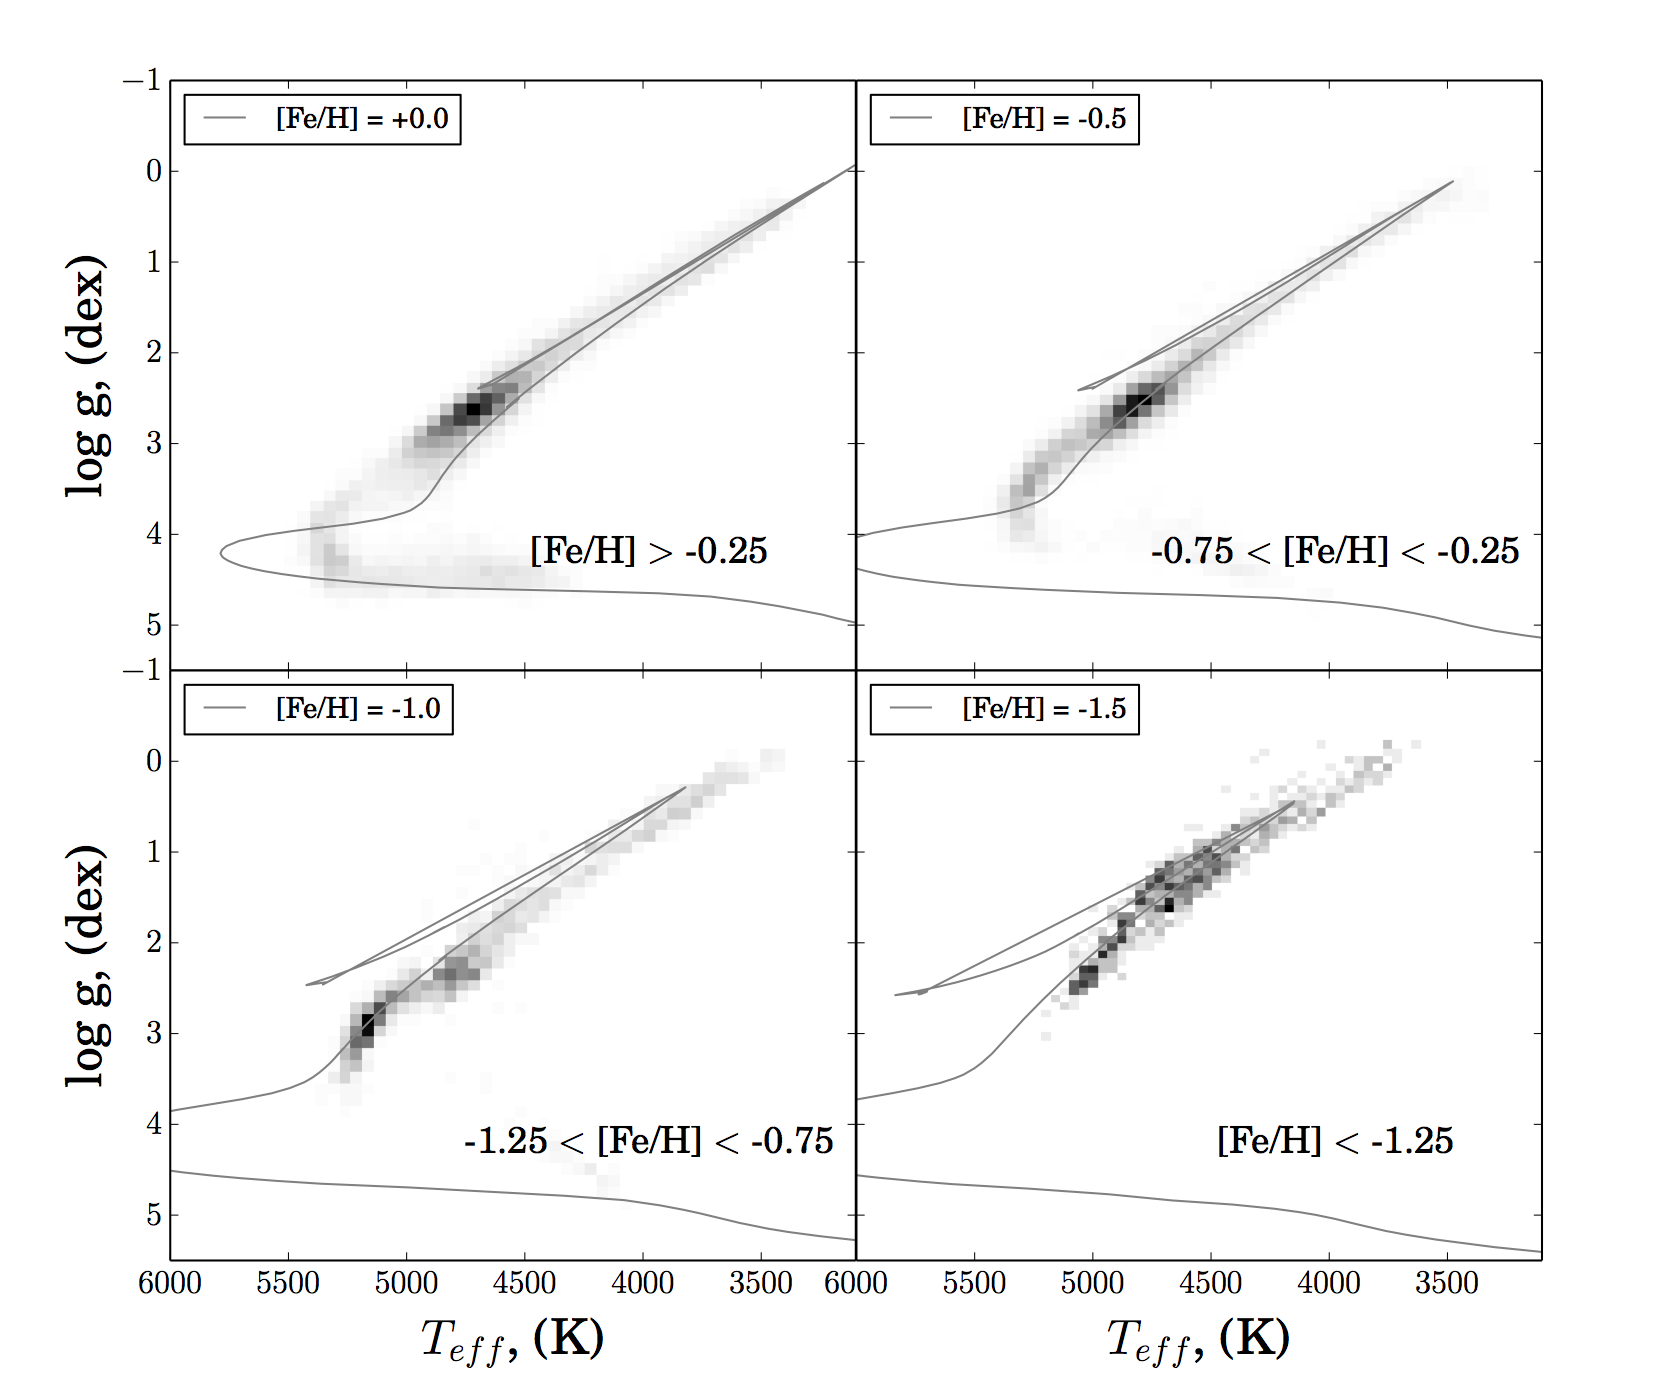
\includegraphics[scale=0.25]{./plots/iso2.png}
  \hspace{-20pt}
    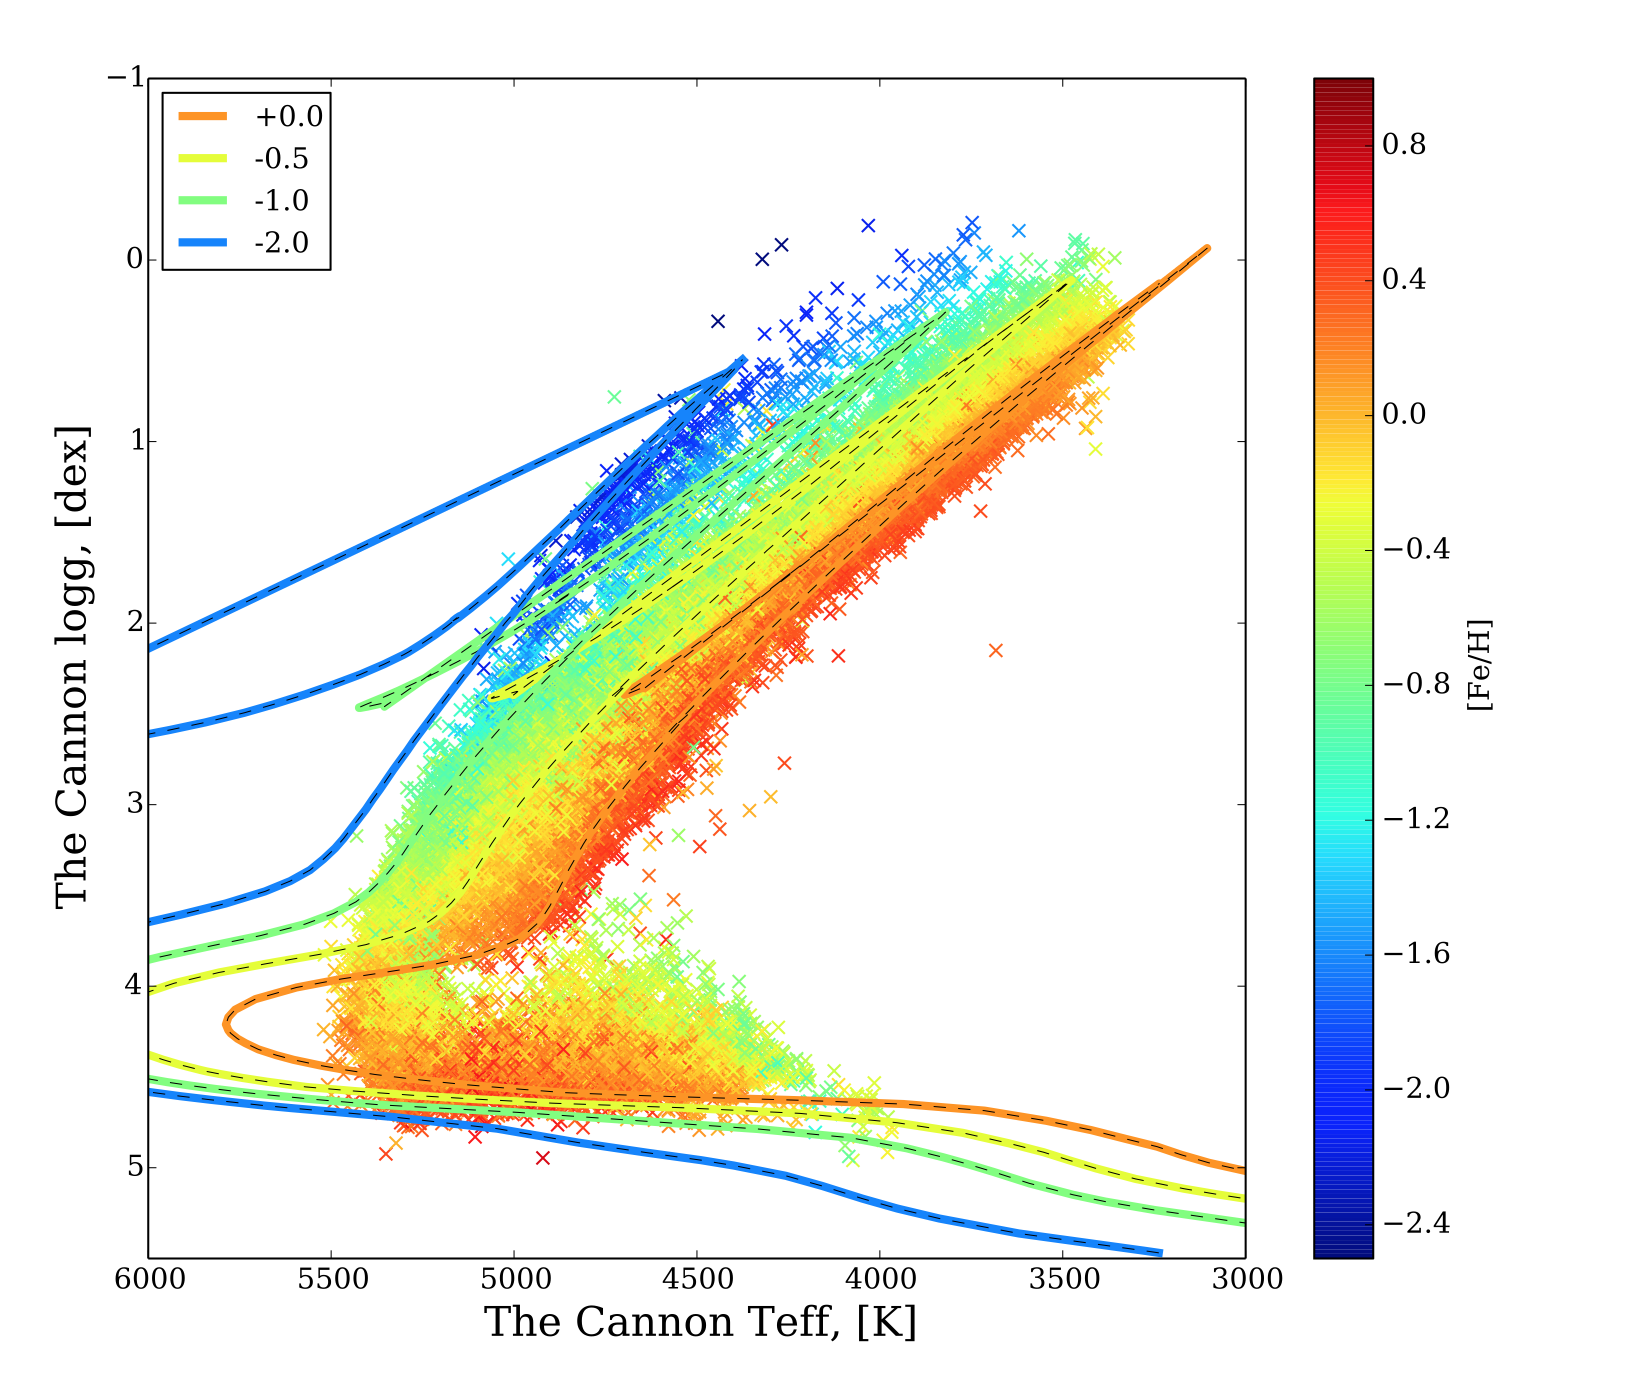
\includegraphics[scale=0.25]{./plots/iso2a.png}
%    \includegraphics[scale=0.33]{./plots/isochrone_mkn20b2.pdf}
\caption{As per Figure \ref{fig:iso} but for the isochrone-corrected'' labels, showing the stars follow the red giant branch on the isochrones.}
\label{fig:iso2}
\end{figure}



\subsection{Anomalous Spectra: Dwarfs and Rotation}

 %run -i makeplot_scatter_test18_coeffs_dwarfs_RevB.py
  \begin{figure}[!h]
   \centering
 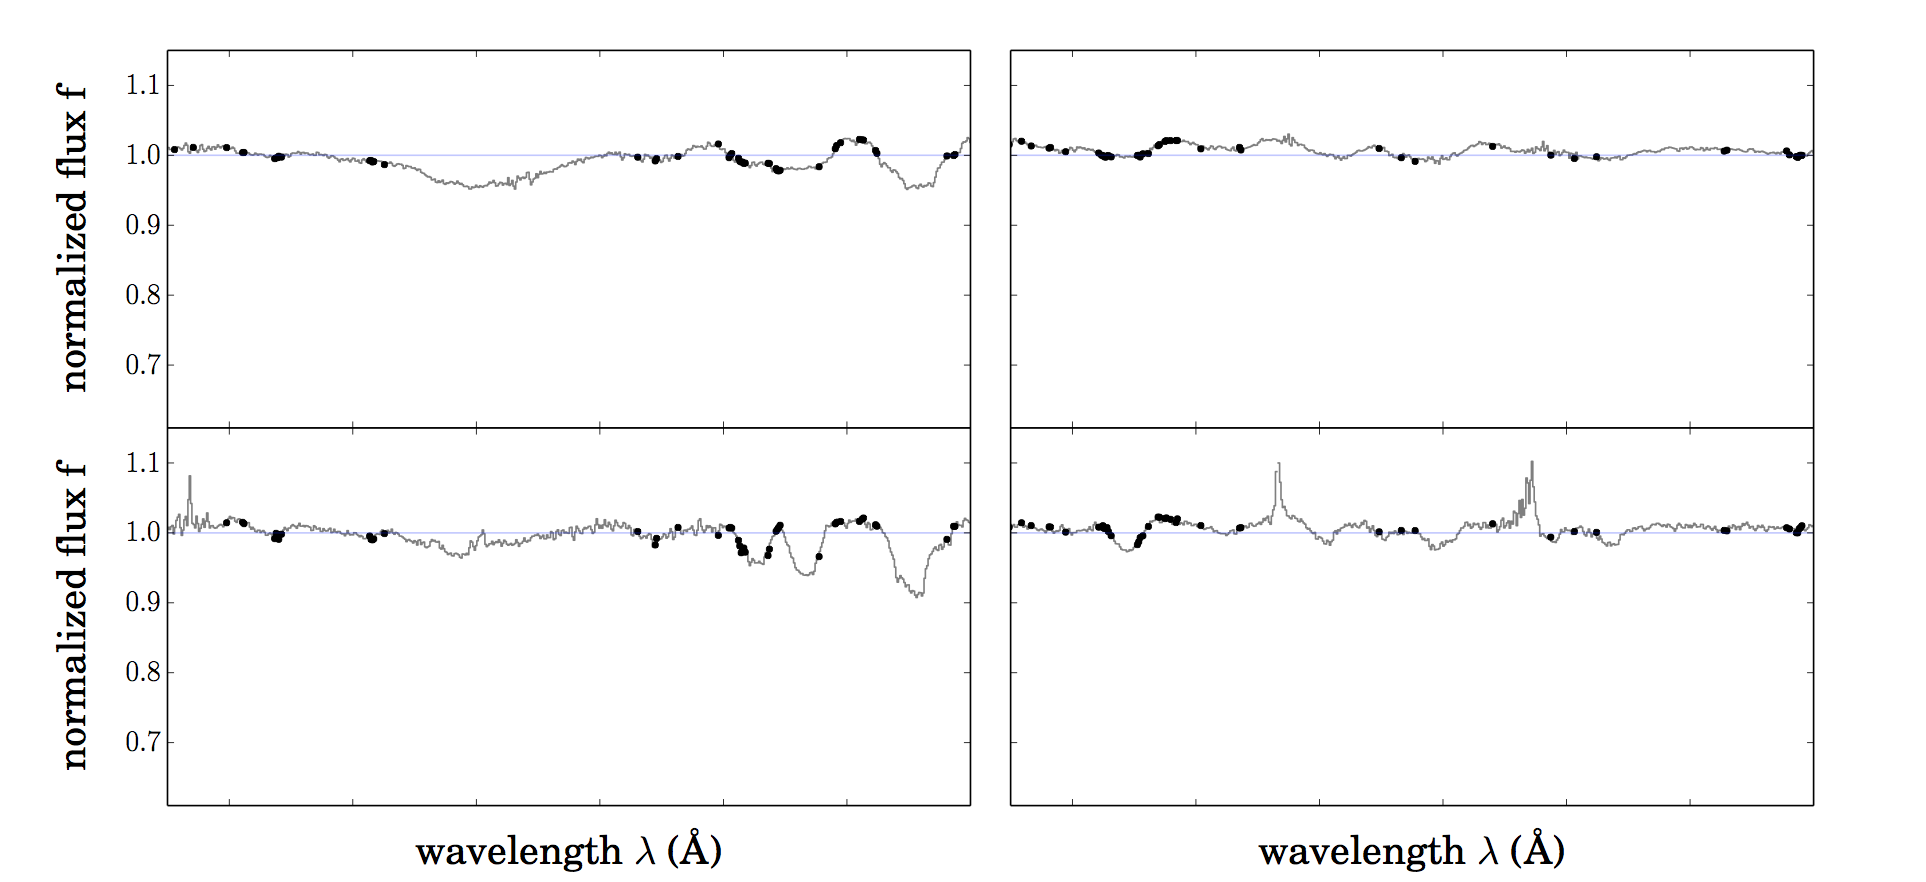
\includegraphics[width=\hsize]{./plots/2dwarfs.png}
  \caption{Examples of hot rotating dwarfs in the \apogee\ DR10 data across regions A and B, comparable to Figure \ref{fig:coeffs}. These types of stars are \textit{not} included in our training data; we can not determine stellar parameters for these stars as they are not captured in our model.}
\label{fig:dwarfs}
\end{figure}


The dwarf spectra in our training set consists of the Pleiades cluster, at a single metallicity. This restricted sample constrains our ability to determine the stellar parameters for dwarf stars. Given these training data, our model \textit{can} differentiate dwarfs from giants, as long as their spectra are comparable to that of the Pleiades. However, none of the dwarfs in our training set are hot rotating objects with broad line features. Three examples of stars with broad line features that are in the test data but not included in our training dataset are shown in Figure \ref{fig:dwarfs}.

It is possible to differentiate these stars with \tc\ because they are output in non-physical space in \teff-\logg, and present as a group of very metal poor, \feh\ $\sim$ --2.0, low \logg\ stars $\sim$ 0, with cool temperatures $\sim$ 4000 K. The metal poor solution determined by \tc\ reflects the dearth of lines in the spectra for these hot stars, given the training model. This group of stars is flagged in \aspcap\ with a \rotwarn\ flag set. We therefore are able to exclude these stars from our analysis using this condition. 
 



 \subsection{Performance at low SNR}


By identifying `true' continuum pixels we have been able to implement a simple continuum normalisation that is robust across low and high SNR, which is valid across the parameter range of our training set. To examine how \tc\ performs at lower SNR, we have taken individual visits from the \apstar\ fits files, when there are $\ge$ 4 visits, and run \tc\ on a single visit spectra which we have continuum-normalised. Note, we have not simply noisifyed the combined visit data for our low SNR tests so this relies on both a robust continuum normalisation and the success of the label-transfer method. Figure \ref{fig:lowsnr} shows a comparison of a sample star for a single visit and combined visits ($>$ 4 total visits). Figure \ref{fig:SNR} presents the results of \tc\ compared to \apogee\ for these stars, showing \textit{only} the \apogee\ stars with errors of $<$ 150 K in \teff\ and $<$ 0.25 dex in \logg, across four SNR intervals, from 20 $<$ SNR $<$ 30 to 100 $<$ SNR $<$ 200. 


These Figures illustrate that the continuum normalisation works well for both of these SNR regimes and is SNR independent, which is not true for a weighted-quantile normalisation. At the highest SNR (and \apogee\ estimates a upper noise floor of 200 although stars do measure above this), the rms difference between \tc\ and \aspcap\ is comparable to the \aspcap\ measurement errors, at 73K in \teff\, 0.18 dex in \logg\ and 0.11 dex in \feh.  At a SNR of 30-50, the rms error increases to 100 K, 0.2 dex and 0.10 dex in \teff, \logg\ and \feh\, respectively. At an SNR of 20-30 the rms error is significantly higher and here the internal errors of \tc\ become comparable to typical minimisation methods and at SNR $<$ 20 exceed them. With this method we can return stellar parameters of \teff, \logg, \feh\ to as good a precisions as minimisation techniques ( \teff\ $<$ 100K, \logg\ $<$ 0.2 dex, \feh\ $< $0.1 dex) with an SNR of $\ge$ 25. 
 
 % run -i makecontin_data1_split.py
 \begin{figure}[!h]
  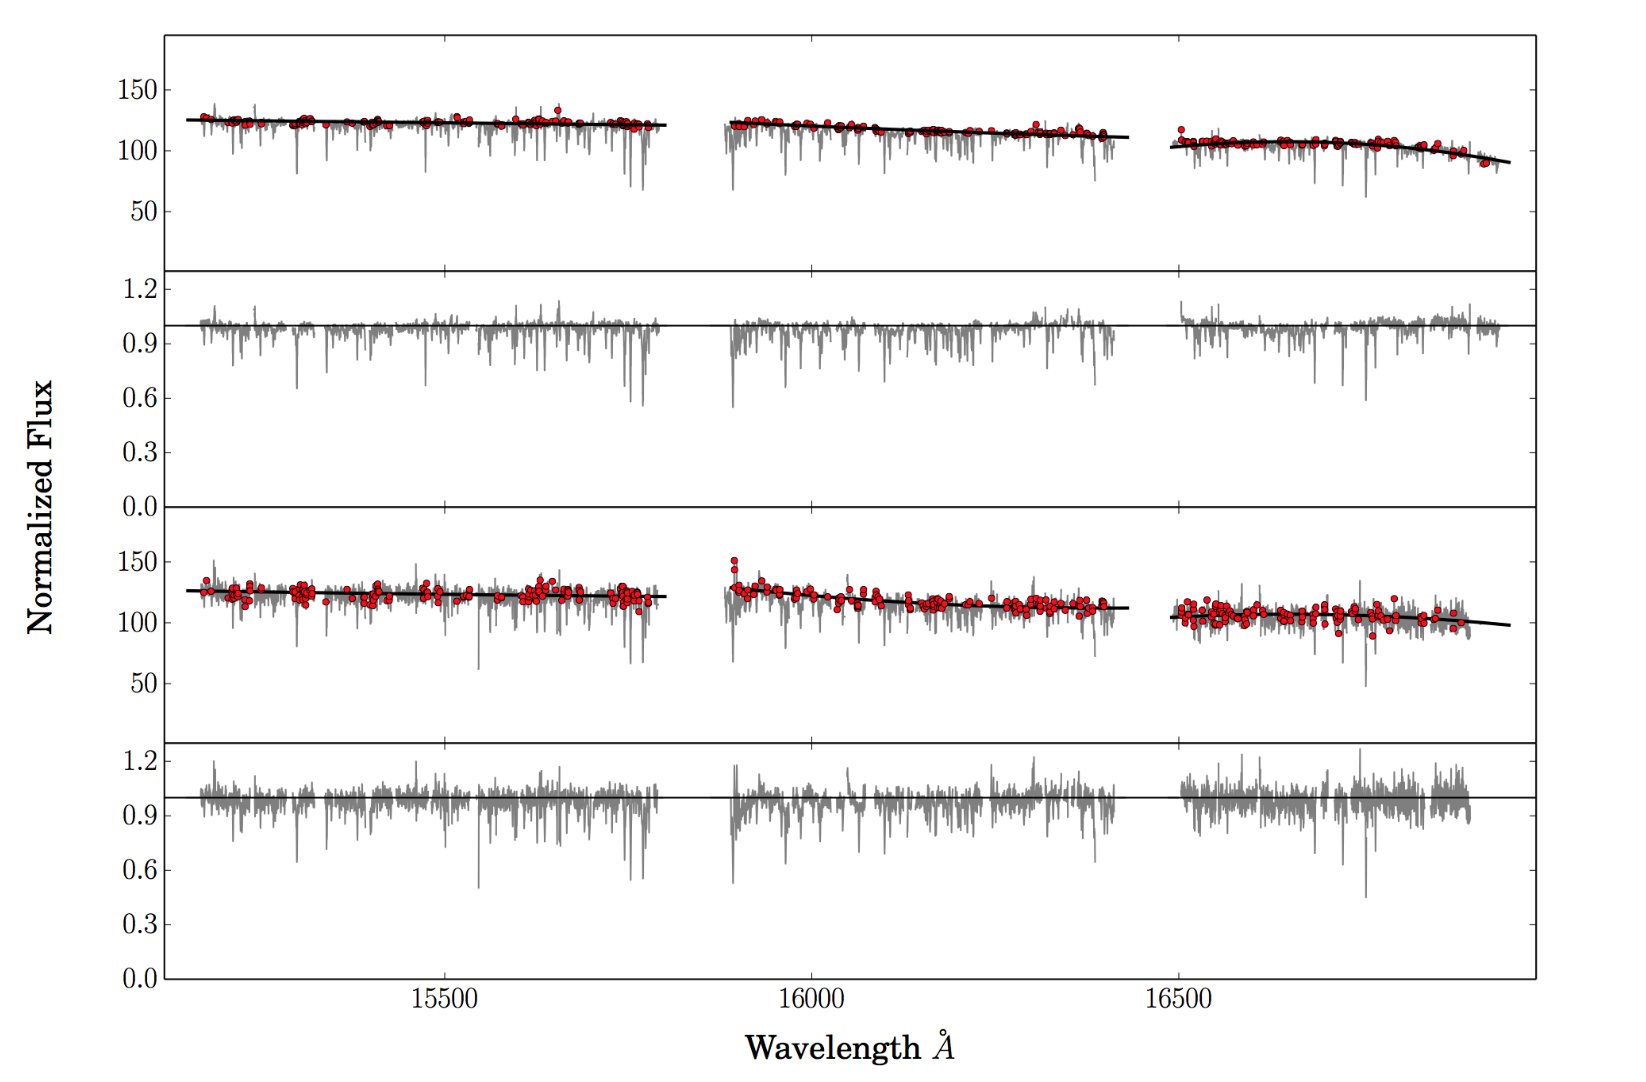
\includegraphics[width=\hsize]{./plots/SNR_continuum3.pdf}
  \caption{Demonstration of the continuum normalisation of the same star at high and low SNR. The \apogee\ reported SNR of the combined visit spectra are SNR = 120 (top two panels) and of the 4th visit shown in the third pane is 25 (bottom two panels). \textbf{mkn: clean up this plot further} }
\label{fig:lowsnr}
\end{figure}

%makeplot_fits_SNRtest.py in /play but changed to makeplot_fits_SNRtest_bw.py
 \begin{figure}[!h]
 \centering
 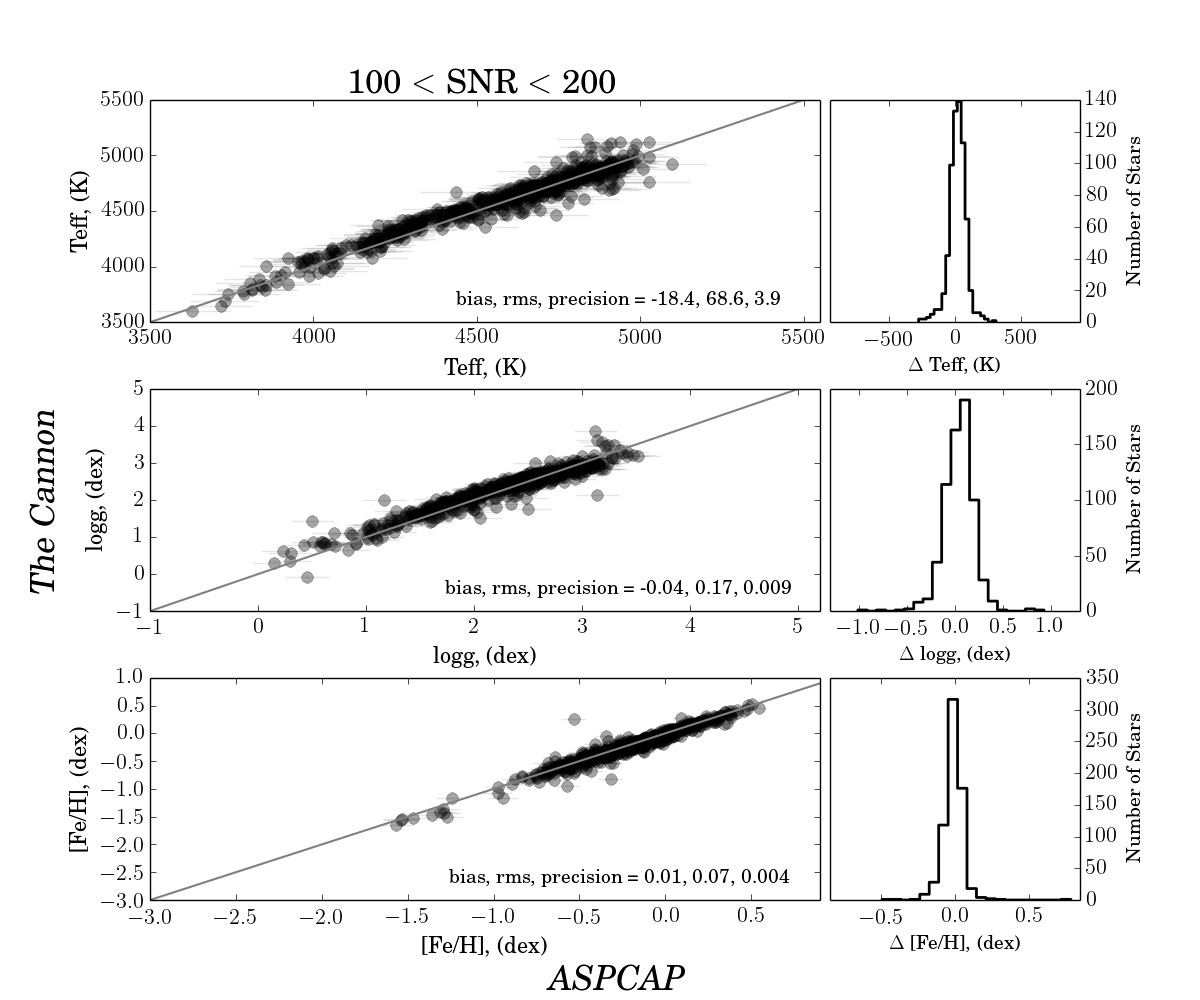
\includegraphics[scale=0.25]{./plots/SNR100to200.png}
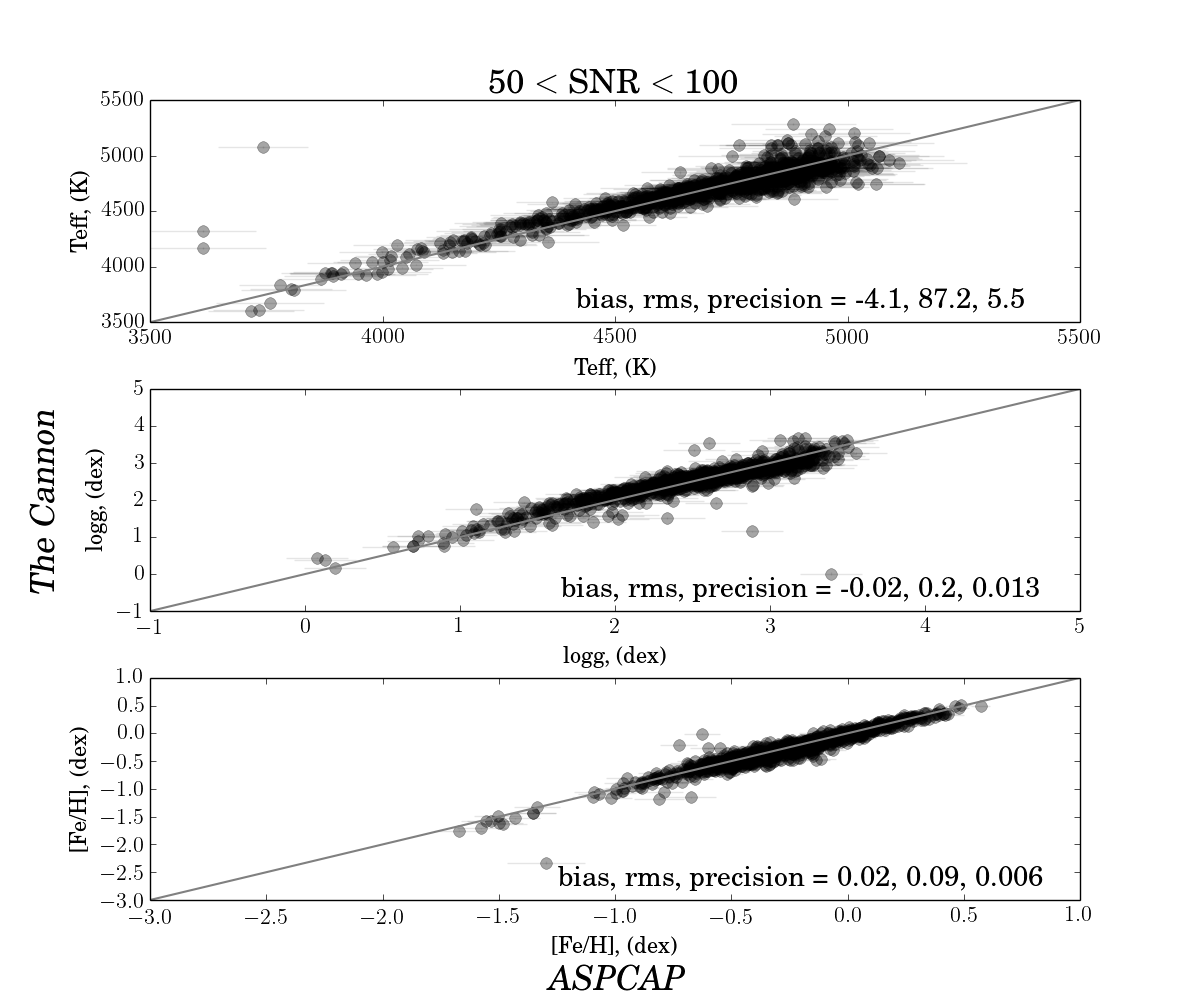
\includegraphics[scale=0.25]{./plots/SNR50to100.png}\\
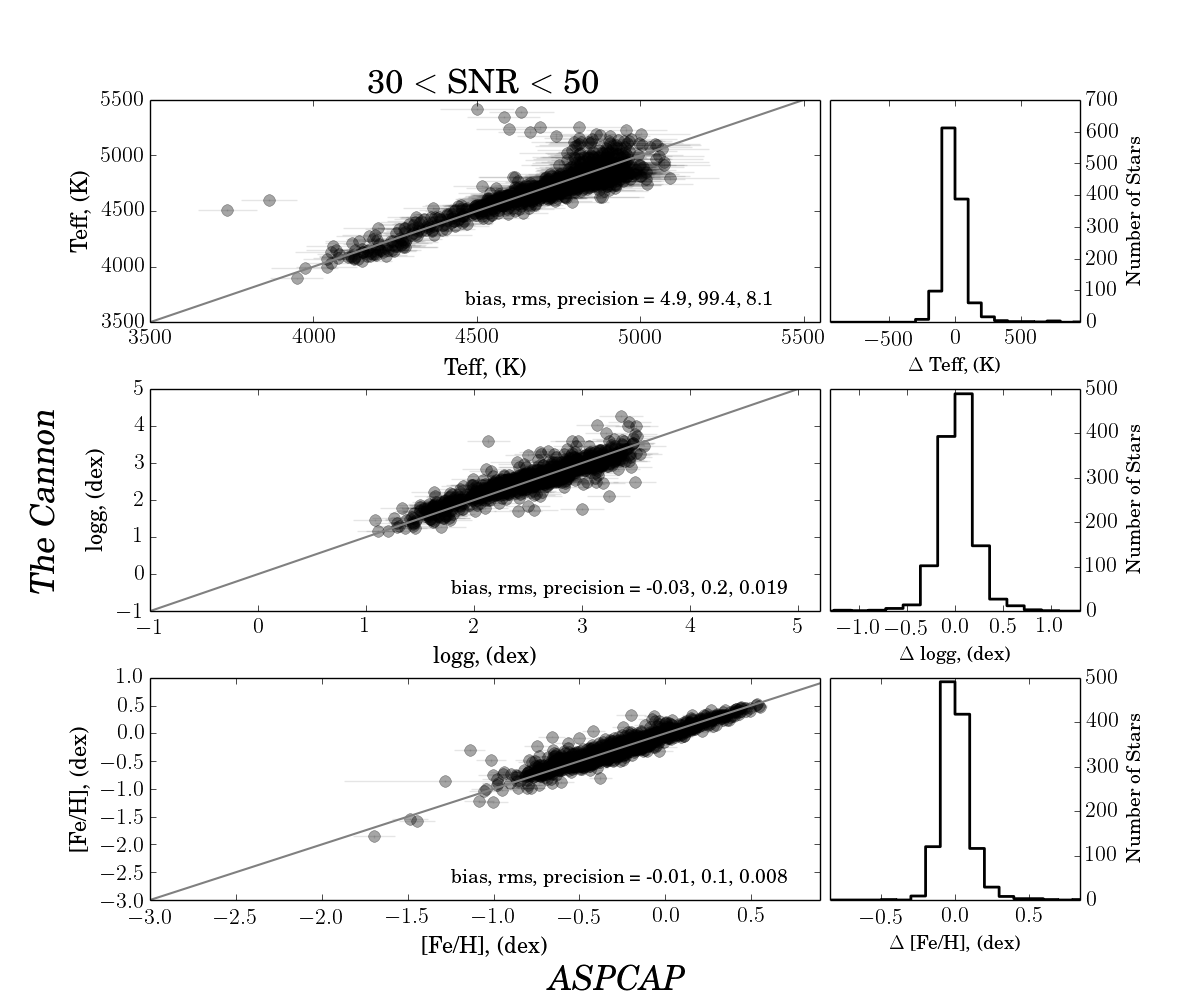
\includegraphics[scale=0.25]{./plots/SNR30to50.png}
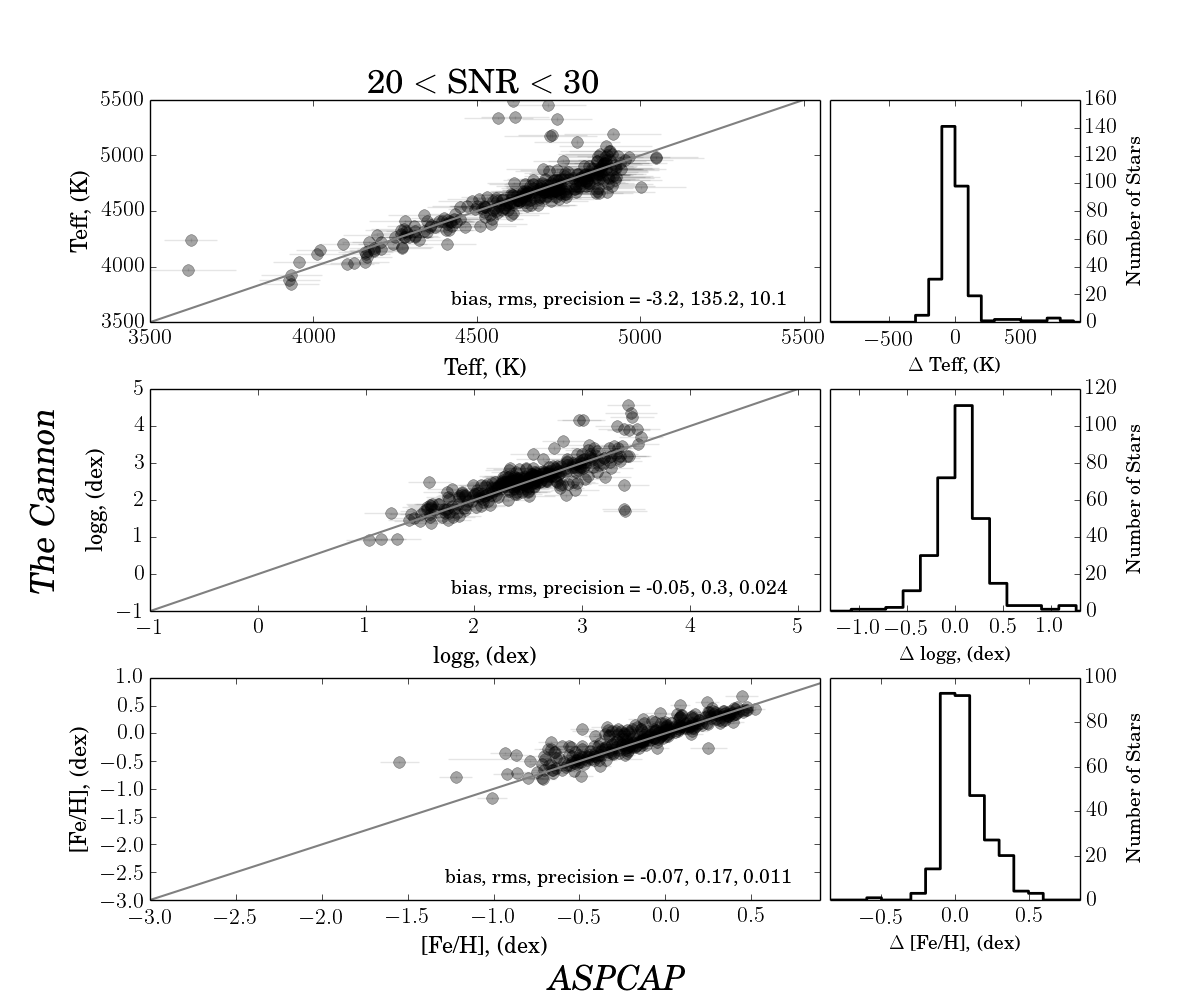
\includegraphics[scale=0.25]{./plots/SNR20to30.png}
    \caption{Four regimes of SNR for single visit spectra. There are 60 stars in the 300 $<$  SNR $<$ 30 bin, 1200 stars in the 30 $<$ SNR $<$ 50 bin, 1100 stars in the 50 $<$ SNR $<$ 100 bin and 670 stars in the 100 $<$  SNR $<$ 200 bin.}
\label{fig:SNR}
\end{figure}

\section{Discussion}

[DWH SAY: THIS PARAGRAPH IS WRONG - MKN SAYS: I changed it] We have demonstrated with \tc,  that using a data-driven model, labels can be transferred from training to test data, simply and efficiently. 
In using a data-driven model which spans the label range of the test data, we do not rely on explicit models in the wavelength region of analysis of the survey. 
We can therefore fully capitalise on large surveys and the information in the data itself, circumvent problems with simplified stellar models , uncertainties in linelists in poorly studied wavelength regions and understand where models are wrong.  

From our implementation of \tc\ on \apogee\ data, we were motivated to examine the calibration space of the labels given the unphysically narrow giant branch returned for DR10 data at low \logg. 
We found by adopting a very naive calibration that shifts the stars to the nearest position on the isochrone from the \aspcap\ value described in Section 2, the stars were returned in a \teff-\logg\ space, across metallicity, in line with expectations of the physical label-space of stars. 
This small \logg\ adjustment is naive, but works well, causing small offsets in the \logg\ scale at low temperatures and \logg\ values compared to the \apogee\ \logg\ input labels, which moves the stars onto the branches or the isochrones. 
This suggests that there is some problem with the input labels in the \logg\ dimension adjusted from Kepler results in DR10. 

For our first implementation of \tc\ presented here, it is trivial to run the almost 60,000 star sample (that is, the size of DR10 from \apogee) through \tc\ on a single laptop, as it takes $<$ 1/10$^{th}$ of a second (on a 2.6 GHz intel core i7) to determine three labels for each star, without any attempt at speed or method optimisation. 
We reproduce the \apogee\ labels, as provided for DR10 in Table 1, without adding any significant uncertainty because we use every pixel in the spectra and have a generative model. 
Our model is comprised of data which represents the probability space of the labels given the physical noise model,  where we let the noise model determine the weighting of the luminosity function, yet we can only do better. 

We have demonstrated that we can work at much lower SNR at least for the three primary stellar parameters with this approach. 
We expect to not gain the same advantage for individual elements with the SNR, but it may be possible to combine elements into subgroups (e.g. alpha, light elements, neutron capture) of covariant spaces \citep[e.g.][]{Ting2012}. In this way we exploit more pixels in the spectra and can operate at significantly lower signal to noise without being penalised in dimensionality of the returned parameter and abundance space. 
This suggests the possibility to dramatically either reduce the cost of survey, or multiply the number of stars observed by a factor of $\ge$ 2 for the same scientific gain. 

In using all of the pixels in the spectrum to obtain the
stellar labels, \tc\ is not dissimilar from the MATrix Inversion for
Spectral SythEsis (\matisse) procedure for derivation of stellar
parameters \citep{RB2006}.
That is, \matisse\ does well at low signal-to-noise for the same
reason as \tc:  They both use the full spectral range.
However, \matisse\ employs a large grid of synthetic spectra and
characterises a set of basis vectors which project onto each observed
spectrum to determine stellar labels by calculating an optimal
combined synthetic spectrum describing the stellar flux.
Conversely, we use a data-driven model and do not project onto any
optimal combined theoretical spectrum.
Rather we directly determine labels using a total of around 80,000
degrees of freedom of information in the data, given the 7200 pixels
comprising the flux and the 10 parameters of the labels in our
implemented model.

[DWH: THERE IS NOTHING SPECIAL OR REQUIRED ABOUT USING ALL THE PIXELS; \tc\ could be generalized to use a linelist or etc.]

 \tc\ is readily expandable to a more general model, a larger training dataset and many more labels which include errors and/or partial characterisation of labels. 
 As it is, our second-order model is hard-coded and extremely restrictive. 
 We currently believe our input labels fully, given they are input without uncertainties, and assume no prior information. 
 We therefore do not take advantage of any physical knowledge that is defined about the phase space the labels can reside in.  
 Furthermore, we currently treat every pixel as independent which is incorrect and therefore builds a physically incomplete model.

 We have barely scratched the surface with what is possible with this methodology given our restricted training dataset, model and labels. 
 Our training dataset itself is clearly too small, comprising only 545 stars including a set of dwarfs at a single metallicity (+0.03 dex). 
 As we lack dwarfs, we can not return parameters in this space to the same precision as giants (\logg\ $\le$ 3.5).  
 We also are missing any dwarfs with rotation in our model and consequently these are returned in an unphysical \teff-\logg\ label-space in the label-transfer. 
 
Although we use \apogee\ as an example, \tc\ can be applied to
any stellar survey.
Details of how the spectra are continuum-normalized might have to be
customized for different surveys, which will have different
line-spread functions and different absorption-line densities, and
therefore different statistics.
In all other respects, however, \apogee\ could be replaced by any spectroscopic
survey that meets the following criteria:
It must contain a set of reference stars with known labels to serve as
a training set.
It must deliver a set of spectra represented on a common rest-frame
wavelength basis.
It must deliver noise variance estimates at every spectral pixel.

The basic implementation of \tc\ presented here considers only three
labels (\teff, \feh, and \logg).
There is nothing fundamental abous this choice; in principle
\tc\ could be extended to consider more labels, or a larger
label space.
For example, a next generation could include [$\alpha$/Fe] or [X/Fe]
labels for elements X.
The only limitation---and it is a \emph{substantial} limitation---is
that as the label-space grows, the training set must grow to fill it;
\tc\ is only as good as its training set.
In general, the training set needs may scale as badly as exponentially
with the dimensionality of the label space, and (as noted above), we
are confident that we don't have enough training stars even now with
a three-dimensional label space.
For this reason, we don't imagine operating \tc\ in the full 30-ish
dimensional label space imagined for the final outputs of surveys like
\apogee\ and \galah; \tc\ is only for establishing the ``first-order'' labels of
greatest importance in setting spectral properties.

In the above, we used a quadratic form for the
relationship between the expected flux and the labels.
This is a choice and can be generalized.
Indeed, the polynomial family is probably not the best family of
functions to be exploring, since they extrapolate badly (edge effects)
and require explicit, qualitative choices about order and cross-terms.
It is probably better to move to a non-parametric form for the functions,
such as Gaussian Processes or similar.
In this case, model complexity would be controlled by continuous
parameters and the functional form could become very complex where the
training data warrant it.
This would be a natural extension of what has been implemented here.

[DWH: SOMETHING ABOUT SPECTRAL REPRESENTATION]

Despite all of this, we have shown using the \apogee\ data that even the simplest model with naive assumptions and an incomplete physical description, works. 
This method is directly transferrable as is, to all other surveys and we expect we would be similarly successful applying this to e.g. \textit{GALAH}, \gaiaeso and 4MOST. 
The success of \tc\ argues for defined stellar standards to effectively transfer labels of benchmark stars, studied at high resolution, to stars in surveys across any wavelength region. 
This would enable all stellar surveys to be unified. 
 
 It is also possible and likely desirable in some cases to implement exactly the same procedure we describe using a synthetic grid instead of data, to train the model. 
 This will remove many of these limitations in the model that are derived from the label-space of the training data labels. However, this also eliminates many of the advantages in a full characterisation of the noise in the data and the true behaviour of labels with flux.
 
 %,  we argue for adopting a wider set of benchmark stars from data in surveys, given labels determined at high resolution, in order to mitigate the issues with limited training datasets. 
 
There are a number of immediate new opportunities with this approach. 
The primary and obvious opportunity is to unify all stellar parameter systems and a key necessity of this is that all common benchmark stars be observed in all surveys. 
The data-driven model approach enables an analysis and characterisation of how and where stellar templates diverge from data, but the ultimate consequence of this methodology is that by using the coefficients of the labels returned in this method for example in our quadratic implementation, we can directly identify and learn \textit{where} the information in a stellar spectrum resides. 
This can be used to make quantitative assessments of the flux dependence on the labels, at the detail of the individual line profiles (asymmetries are clear, a depth versus width versus wings of the features is clear) and, for example, determine continuum pixels as we have done to obtain a robust continuum normalisation across SNR. 
The information in the spectra  is a direct output from the model, which is immensely more informative than the reverse assumption of assessing regions of interest as informed by linelists.  
\tc\ is therefore extremely relevant for chemical tagging and we take an approach of a data-driven differential analysis of spectra, by characterising the behaviour of flux and labels, as a way to fingerprint stars with a common formation history.

A direct first additional upgrade for \tc\ aligned with directing this method toward chemical tagging, which large surveys like \galah\ and \apogee\ have been constructed around,  is  to add more labels.
 An obvious initial choice is $\alpha$-enhancement and a subset of key individual abundances [X/Fe]. 
 It is even possible to test what, if any, information in the spectra are correlated with an age label. 
 If such information is present in the spectra across a large set of stars in a survey, this method \textit{will} determine exactly which pixels are responsible for carrying this information. In addition, we will gain significantly by moving to a more flexible model like a Gaussian process and allowing our model to be informed by priors in these new directions for this work. 

[DWH SAY:  THE DISCUSSION (above) IS A BIT REPETITIVE; WE CAN PROBABLY COMBINE AND SHORTEN PARAGRAPHS ABOUT GENERALIZATIONS.]

\textbf{DWH can you expand on generative models: data-driven model that represents the noise -  very successful as it respects the noise model. generative - synth, L.F. - permits discovery, interpretation.}


\section*{ Acknowledgements}

The name \tc\ is inspired by the astronomer Annie Jump Cannon,
who was the pioneer on stellar classification without physical models!
We would like to thank Daniel Foreman-Mackey (NYU), 
Morgan Fouesneau, Jon Holtzman,  Keivan Stassun and Jennifer Johnson
for valuable discussions.
DWH was partially supported by
the NSF (grant IIS-1124794), NASA (grant NNX08AJ48G), and the
Moore--Sloan Data Science Environment at NYU.
The research has received funding from the European Research Council under the European
Union's Seventh Framework Programme (FP 7) ERC Grant Agreement n.
[321035].

Funding for SDSS-III has been provided by the Alfred P. Sloan Foundation, the Participating Institutions, 
the National Science Foundation, and the U.S. Department of Energy Office of Science. The SDSS-III web site is $http://www.sdss3.org/.$\\

Funding for SDSS-III has been provided by the Alfred P. Sloan Foundation, the Participating Institutions, the National Science Foundation, and the U.S. Department of Energy Office of Science. The SDSS-III web site is $http://www.sdss3.org/.$\\

SDSS-III is managed by the Astrophysical Research Consortium for the Participating Institutions of the SDSS-III Collaboration
 including the University of Arizona, the Brazilian Participation Group, Brookhaven National Laboratory, Carnegie Mellon University, 
 University of Florida, the French Participation Group, the German Participation Group, Harvard University, the Instituto de Astrofisica 
 de Canarias, the Michigan State/Notre Dame/JINA Participation Group, Johns Hopkins University, Lawrence Berkeley National Laboratory, 
 Max Planck Institute for Astrophysics, Max Planck Institute for Extraterrestrial Physics, New Mexico State University, New York University, 
 Ohio State University, Pennsylvania State University, University of Portsmouth, Princeton University, the Spanish Participation Group, 
 University of Tokyo, University of Utah, Vanderbilt University, University of Virginia, University of Washington, and Yale University


\bibliography{tc3.bib}


\end{document}
